%% LaTeX2e class for student theses
%% thesis.tex
%% 
%% Karlsruhe Institute of Technology
%% Institute for Program Structures and Data Organization
%% Chair for Software Design and Quality (SDQ)
%%
%% Dr.-Ing. Erik Burger
%% burger@kit.edu
%%
%% See https://sdq.kastel.kit.edu/wiki/Dokumentvorlagen
%%
%% Version 1.4, 2023-06-19

%% Available page modes: oneside, twoside
%% Available languages: english, ngerman
%% Available modes: draft, final (see README)
\documentclass[twoside, english]{sdqthesis}

%% ---------------------------------
%% | Information about the thesis  |
%% ---------------------------------

%% Name of the author
\author{Jan Knoblich}

%% Title (and possibly subtitle) of the thesis
\title{Evaluation of Intel Confidential Computing Technologies with Regard to their Performance, Security and Resulting Application Possibilities}

%% Type of the thesis 
\thesistype{Bachelor's Thesis}

%% Change the institute here, ``KASTEL'' is default
\myinstitute{KASTEL – Institute of Information Security and Dependability
Cryptography and Security Group}

%% You can put a logo in the ``logos'' directory and include it here
%% instead of the SDQ logo
% \grouplogo{myfile}
%% Alternatively, you can disable the group logo
% \nogrouplogo

%% The reviewers are the professors that grade your thesis
\reviewerone{Prof. Dr. Jörn Müller-Quade}
\reviewertwo{Prof. B}

%% The advisors are PhDs or Postdocs
\advisorone{Jeremias Mechler, M.Sc. }
%% The second advisor can be omitted
\advisortwo{Felix Dörre, M.Sc.}

%% Please enter the start end end time of your thesis
\editingtime{17. October 2023}{12. March 2024}

\settitle

%% --------------------------------
%% | Bibliography                 |
%% --------------------------------

%% Use biber instead of BibTeX, see README
\usepackage[citestyle=numeric,style=numeric,backend=biber]{biblatex}
\addbibresource{thesis.bib}

%% For example texts -- please remove in the final version
\usepackage[acronym]{glossaries}
\usepackage{todonotes}
\usepackage{listings}

\usepackage{bera}
\usepackage{xcolor}
\usepackage[T1]{fontenc}
\usepackage{array}

\colorlet{punct}{red!60!black}
\definecolor{background}{HTML}{EEEEEE}
\definecolor{delim}{RGB}{20,105,176}
\definecolor{black}{RGB}{0,0,0}
\colorlet{numb}{magenta!60!black}

\lstdefinelanguage{jsonmain}{
    basicstyle=\small\ttfamily,
    numbers=left,
    numberstyle=\scriptsize,
    stepnumber=1,
    numbersep=8pt,
    showstringspaces=false,
    breaklines=true,
    frame=lines,
    backgroundcolor=\color{background},
    literate=
     *{0}{{{\color{black}0}}}{1}
      {1}{{{\color{black}1}}}{1}
      {2}{{{\color{black}2}}}{1}
      {3}{{{\color{black}3}}}{1}
      {4}{{{\color{black}4}}}{1}
      {5}{{{\color{black}5}}}{1}
      {6}{{{\color{black}6}}}{1}
      {7}{{{\color{black}7}}}{1}
      {8}{{{\color{black}8}}}{1}
      {9}{{{\color{black}9}}}{1}
      {:}{{{\color{punct}{:}}}}{1}
      {,}{{{\color{punct}{,}}}}{1}
      {\{}{{{\color{delim}{\{}}}}{1}
      {\}}{{{\color{delim}{\}}}}}{1}
      {[}{{{\color{delim}{[}}}}{1}
      {]}{{{\color{delim}{]}}}}{1},
}
\lstdefinelanguage{json}{%
  language     = jsonmain,
  basicstyle=\footnotesize\ttfamily,
  numbers=none,
}
\usepackage{cleveref}

\newglossaryentry{SEAM}
{
    name=secure arbitration mode,
    description={A new x86 execution mode designed to isolate the TDX module and SEAMLDRs from entities outside the TDX TCB}
}

\newglossaryentry{NP-SEAMLDR1}
{
    name=Non Persistent SEAM Loader,
    description={The root-of-trust for Intel TDX. This signed module bootstraps the P-SEAMLDR.}
}
\newglossaryentry{P-SEAMLDR1}
{
    name=Persistent SEAM Loader,
    description={Authenticates and installs (or uninstalls) the TDX module}
}

\newglossaryentry{TDX Module}
{
    name=TDX Module,
    description={The software component which manages TDs. The VMM directs it and exposes both guest-facing and VMM-facing APIs}
}

\newglossaryentry{GETSEC}
{
    name=GETSEC instructions,
    description={The instructions with which SMX is implemented in Intel architectures}
}
\newglossaryentry{TCB}
{
    name=TCB,
    description={The trusted computing base}
}
\newglossaryentry{SEAMRR}
{
    name=SEAMRR,
    description={The memory region where the TDX module and control structures are located}
}

\newglossaryentry{TD}
{
    name=TD,
    description={A trusted domain is a hardware-isolated VM using the TDX architecture}
}



\newacronym{tcb}{TCB}{Trusted Computing Base}
\newacronym{td}{TD}{Trusted Domain}
\newacronym{tdx}{TDX}{Trusted Domain Extensions}
\newacronym{NP-SEAMLDR}{NP-SEAMLDR}{\Gls{NP-SEAMLDR1}}
\newacronym{P-SEAMLDR}{P-SEAMLDR}{\Gls{P-SEAMLDR1}}
\newacronym{OS}{OS}{Operating System}
\newacronym{CCC}{CCC}{Confidential Computing Consortium}
\makeglossaries


%% ====================================
%% ====================================
%% ||                                ||
%% || Beginning of the main document ||
%% ||                                ||
%% ====================================
%% ====================================
\begin{document}
\listoftodos



%% Set PDF metadata
\setpdf

%% Set the title
\maketitle

%% The Preamble begins here
\frontmatter

%% LaTeX2e class for student theses: Declaration of independent work
%% sections/declaration.tex
%% 
%% Karlsruhe Institute of Technology
%% Institute for Program Structures and Data Organization
%% Chair for Software Design and Quality (SDQ)
%%
%% Dr.-Ing. Erik Burger
%% burger@kit.edu
%%
%% Version 1.4, 2023-06-19

\thispagestyle{empty}
\null\vfill
\noindent\hbox to \textwidth{\hrulefill} 
%
% Gemäß Studien- und Prüfungsordnung Bachelor Informatik des KIT,
% § 14 (5) vom 10.05.2022
% 
\iflanguage{english}{I declare that I have developed and written the enclosed
thesis completely by myself. 
I have not used any other than the aids that I have mentioned. 
I have marked all parts of the thesis that I have included from 
referenced literature, either in their original wording or paraphrasing their
contents. 
I have followed the by-laws to implement scientific integrity at KIT.}%
{Ich versichere wahrheitsgemäß, die Arbeit selbstständig verfasst, alle benutzten 
Quellen und Hilfsmittel vollständig und genau angegeben und alles kenntlich gemacht 
zu haben, was aus Arbeiten anderer unverändert oder mit Abänderungen entnommen wurde 
sowie die Satzung des KIT zur Sicherung guter wissenschaftlicher Praxis in der 
jeweils gültigen Fassung beachtet zu haben. }
 
 
%% ---------------------------------------------
%% | Replace PLACE and DATE with actual values |
%% ---------------------------------------------
\textbf{Karlsruhe, }
\vspace{1.5cm}
 
\dotfill\hspace*{8.0cm}\\
\hspace*{2cm}(\theauthor) 
\cleardoublepage

\setcounter{page}{1}
\pagenumbering{roman}

%% ----------------
%% |   Abstract   |
%% ----------------
 
%% For theses written in English, an abstract both in English
%% and German is mandatory.
%%
%% For theses written in German, a German abstract is sufficient.
%%
%% The text is included from the following files:
%% - sections/abstract

\includeabstract


%% ------------------------
%% |   Table of Contents  |
%% ------------------------
\tableofcontents


\printglossaries

\listoffigures
\listoftables

%% -----------------
%% |   Main part   |
%% -----------------

\mainmatter
\newcommand{\myparagraph}[1]{\paragraph*{#1}\mbox{}\\}
\newcommand{\guillemet}[1]{\guillemotleft #1 \guillemotright}
%% LaTeX2e class for student theses
%% sections/content.tex
%% 
%% Karlsruhe Institute of Technology
%% Institute for Program Structures and Data Organization
%% Chair for Software Design and Quality (SDQ)
%%
%% Dr.-Ing. Erik Burger
%% burger@kit.edu
%%
%% Version 1.4, 2023-06-19

\chapter{Introduction}
\label{ch:Introduction}

\begin{fancyquotes}
Privacy is not something that I’m merely entitled to, it’s an absolute prerequisite. 

\textit{Marlon Brando}
\end{fancyquotes}

Privacy becomes increasingly more prevalent in times, where we put more and more information about ourselves on the Internet. While many people give no regard to the amount of data they put onto the internet for free, this thesis will focus less on what people are willingly sharing but how to protect data that we want to protect. Data can usually be in one of three states requiring protection. Proven procedures for the secure transmission and storage of data have existed for some time. In the past, however, it was a challenge to fully protect data from unauthorized access during processing. This situation has changed fundamentally over the last ten years. Confidential computing refers to concepts and technologies that are designed to protect data and applications, even if they are executed on third-party hardware. This thesis focuses on Intel's \Gls{TDX} from 2023, an extension of the Software Guard Extension (SGX) from 2015. These offer developers the option of using hardware-based encryption. In the case of SGX, selected memory areas and application code are isolated; \Gls{TDX} extends this to include hardware-based isolation of the entire virtual machine (VM) from the hypervisor, among other things. 
A fundamental problem in the security industry is the trade-off between performance and security. For this reason, this bachelor thesis is dedicated to analyzing the impact of using these technologies on the performance of a Large Language Model (LLM). This thesis contributes to this goal by answering the following questions:
\begin{itemize}
    \item What is the impact of \Gls{TDX} on an applications performance? How do they compare to general performance decreases of using an application in a VM?
\item What security assumptions need to be made for a system using Intel \Gls{TDX} to be secure? What does it take to securely connect to a TD and what risks still remain?
\end{itemize}
To answer these two questions, the \Gls{TDX} specifications and attestation flow was investigated and explained. The limits of the threat model that is in use by Intel and the Confidential Computing Consortium were outlined, this was followed by looking at a practical implementation of a TD, its quote generation and general attestation flow. This data was then used to differentiate between the theoretical and practical dangers of \Gls{TDX}.
To answer the performance questions, numerous benchmarks were run using Python and Huggingface transformers on Intel Xeon 8460H CPUs in the Intel Developer cloud.
The color schemes in this thesis are chosen to be readable by as many people as possible, including if shown in black and white. If viewed in color by a person who does not experience colorblindness, they might look weird for that reason.

\chapter{Preliminaries}
\label{ch:Foundations}

\section{Confidential Computing}
\label{sec:Foundations:ConfComputing}
Confidential Computing means the protection of data during computation by performing those computations in attested Trusted Execution Environments (TEE). Similarly to Trusted Computing, Confidential Computing is predominantly a marketing term and has no single definition. The following tries to establish the definition as it will be used in this thesis. Unlike Trusted Computing, which aims to establish integrity of hardware and software, Confidential Computing also aims to guarantee the authenticity. Using TEEs in the lowest layer of hardware reduces the number of trusted parties. In this case, a party could be a hardware or software vendor. Security in one abstraction layer of the compute stack is only as strong as the layers below it if no other measures are used to prevent access. Homomorphic encryption gives some additional security guarantees even if the underlying layers are not trusted. Figure \ref{fig:computestack} shows a basic compute stack. A bug in the hypervisor, if present, can affect the execution of the operating system and, in the worst case read or change the data in use.
\begin{figure}
\centering
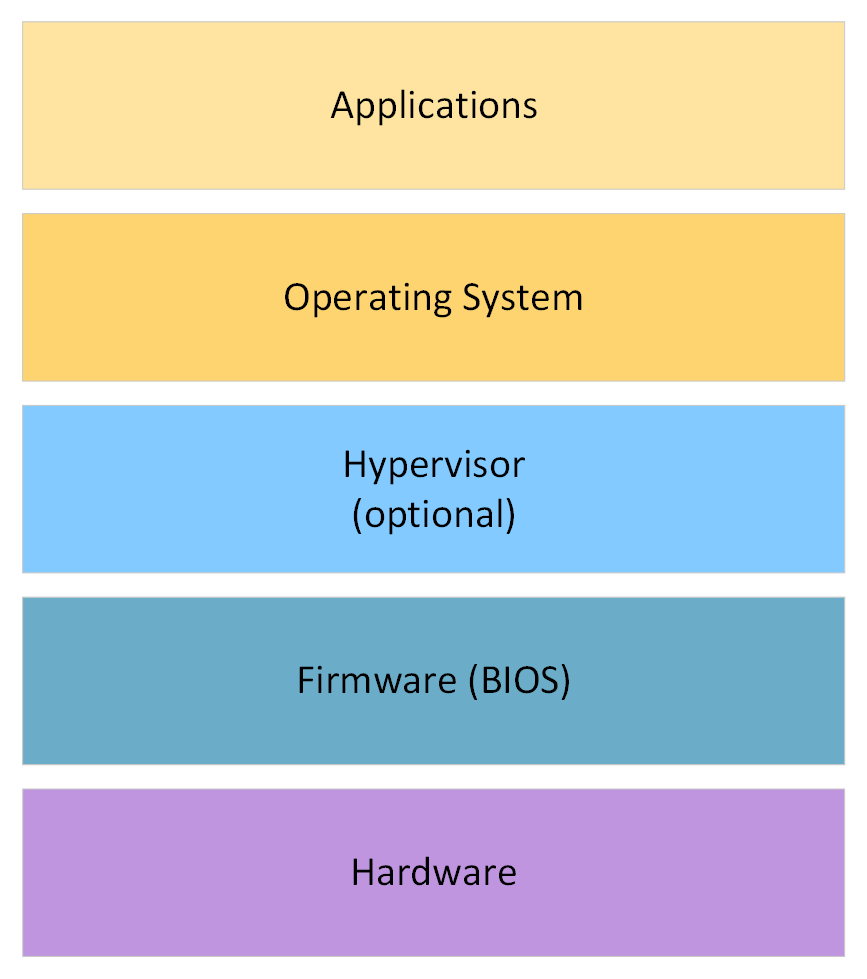
\includegraphics[width=0.5\textwidth]{figures/ComputeStack.png}
\caption{A rudimentary Compute Stack. Most layers can be split up further if needed to}
\label{fig:computestack}
\end{figure}Security in higher layers can be bypassed from lower layers. Security solutions at the hardware level can remove the operating system, device drivers, and more from the list of trusted parties. Confidential Computing protects data in use by performing computation in a hardware-based Trusted Execution Environment (TEE). A TEE is, as defined by the Confidential Computing Consortium, an environment that provides assurance in three different properties:
\begin{itemize} 
    \item \guillemotright Data confidentiality: Unauthorized entities cannot view data while it is in use within the TEE
    \item Data integrity: Unauthorized entities cannot alter the data while it is in use within the TEE.
    \item Code integrity: Unauthorized entities cannot alter the code executing in the TEE.\guillemotleft \cite{noauthor_ccc_outreach_whitepaper_updated_november_2022pdf_2023}
\end{itemize} 
In the context of Confidential Computing, unauthorized entities include, but are not limited to, other applications on the host, the host operating system itself, as well as the hypervisor, the infrastructure owner, and anyone else with physical hardware access. 
Combined, these three attributes provide an assurance that the data are kept confidential and the calculations that are performed are correct.
Depending on the specific TEE used, there might be additional security properties, but the TEEs covered in this thesis do not have more\cite{noauthor_ccc_outreach_whitepaper_updated_november_2022pdf_2023}.

Integrity Measurement Architecture (IMA) is a feature of the Linux kernel that ensures system integrity while the system is running. It computes the hashes of files and programs prior to their execution, provides reporting capabilities, and verifies that they adhere to a predefined list.\cite{Luo_container_ima}. IMA is recommended by the TCG for identity verification \cite{TCG Guidance on Integrity Measurements and Event Log Processing}. According to the IMA wiki \url{https://sourceforge.net/p/linux-ima/wiki/Home/} it contains two subsystems: Measurement and Appraisal. Measurement is responsible for gathering, storing, and verifying measurements. Appraisal conducts the evaluation and auditing tasks by comparing a collected hash with a stored hash and prevents access if they do not match. IMA depends on Trusted Platform Module (TPM)\cite{Luo_container_ima}. 

\section{Trusted Domain Extension}
One implementation of TEEs by Intel is called Trusted Domain Extensions (TDX). This section gives an overview of its building blocks, its system architecture, memory protection mechanisms, I/O model, attestation, and future features.
\subsection{TDX Building Blocks}
\label{sec:tdxBuildingBlocks}
TDX combines and extends several existing Intel technologies, including Virtualization Technology (VT), Total Memory Encryption (TME), and Software Guard Extensions (SGX). This section will provide a brief overview of the technologies and how they are used. The building blocks were also outlined in \cite{cheng_intel_2023}, to which this will give some more context.
\subsubsection{Software Guard Extension}
SGX is a set of instruction codes, which were Intels first trusted execution environment. It was intended to protect against memory bus snooping and cold boot attacks. It is still in use today to protect code and data within a so called enclave, which is a secure container, containing sensitive code and data. It can contain entire applications or even an operating system but was intended to house just small parts of an application. It is encrypted using Memory Protection Extensions a predecessor to TME explained in \cref{Memory Encrpytion}. Data is only decrypted inside the processor\cite{intel_corporation_overview--intel-sgx-enclave_nodate}. SGX aims to protect the integrity and confidentiality of the computation inside an enclave. The RAM of an enclave can only be accessed by authorized code. SGX uses hardware-based memory encryption to protect the enclave. Any unauthorized attempt to access the memory will result in an exception. SGX offers both local and, more importantly, remote attestation to verify the integrity of enclaves. Local attestation establishes trust between two local enclaves, and remote attestation verifies trustworthiness to a third party entity. More on attestation can be found in \cref{TDX attestation} On the same platform, TDX and SGX are within the same Trusted Computing Base (TCB).  Therefore, they can attest each other locally\cite{intel_corporation_intel_2024-1}, which will become important for TDX in \cref{Pre-Attestation setup}. During its lifetime Intel SGX has had many security issues, with most of them being preventable by the application developer themself. \url{https://sgx.fail/}\cite{sgxfail} provides an overview of known issues at the time of writing and ways to mitigate them. The same source also contains an overview of attacks that can only be prevented with microcode updates by Intel itself. SGX does not want to protect against hardware-based attacks in general\cite{costan_intel_2016}. It wants to protect against unpriviliged and privileged software attacks as well as startup code attacks \cite{schutz_general_nodate}.
\subsubsection{Intel Virtualization Technology}
Intel Virtualization Technology (Intel VT) is a set of hardware-assisted virtualization features in Intel processors that can provide improved performance, isolation, and security compared to software-based virtualization. Intel VTs features include virtualization of the CPU, memory, I/O.
Intel processors contain, depending on the architecture, either VT-x or VT-i instructions. The latter being only used on the discontinued Itanium architecture. Processors with VT-x have a special instruction set called Virtual Machine Extensions (VMX), which enables virtualization control. Virtualization allows the usage of multiple isolated Virtual Machines on the same hardware. It can also allow multiple different operating systems to run in these VMs\cite{intel_corporation_intel_nodate}. VMX has two different execution modes: VMX root mode, used by the hypervisor, and VMX nonroot mode, used by the guest VMs. VMX uses a second-level address translation called Extended Page Table (EPT), which aims to eliminate the overhead from software-managed page tables \cite{uhlig_intel_2005}. The TDX Module (TDXM) runs in the new Secure Arbitration Mode (SEAM) VMX root and the TDs run in the nonroot mode. The biggest change from normal VMX to SEAM VMX is the usage of an additional Extended Page Table. With VMX the hypervisor holds only one table per guest kernel, the TDXM has two per guest TD. A protected one for private memory and another unprotected one for shared memory.
With TDX being a virtual machine-based TEE, it depends on VT to ensure isolation between its Trusted Domains (TDs)\cite{cheng_intel_2023}.
\subsubsection{Intel Total Memory Encryption}
\label{Memory Encrpytion}
Intel Total Memory Encryption (TME) is a security measure designed to protect against attackers who have physical access to the memory of a computer or direct access via a host system and attempt to steal data. TME aims to protect against some, for example bus memory probing, but not all physical attacks, for example Direct Memory Access attacks.TME encrypts the entire computer's memory using a single key, which is generated at boot-time by a hardened hardware-based random number generator. Memory encryption is performed by encryption engines on each memory controller, using the recommended standard AES-XTS, for storage encryption, of the US National Institute of Standards and Technologies \cite{morris_dworkin_recommendation_2015} and the German Federal Office for Information Security with 128 or 256-bit keys\cite[~p. 24]{bundesamt_fur_sicherheit_in_der_informationstechnik_cryptographic_2023}. The encryption engines sit directly in between the memory controllers and the CPU cache, meaning the data inside the SoC remains plain text, while the data inside the memory is always encrypted. Total Memory Encryption Multi Key (TME-MK, also sometimes MKTME) extends TME to support multiple keys and memory encryption at page granularity. To use TME-MK in virtualized environments, the hypervisor must be trusted, which violates the threat model for confidential computing, which will be explained in more detail in chapter \ref{Security Analysis}. Therefore, in TDX, the TDX Module is responsible for controlling the memory encryption of TDs. Figure \ref{fig:component-overview} shows what a TD encapsulates. The TDX Module requests the processor to generate a new key when building a new TD and binds the two together via its Key Management Tables. The TDX module then utilizes MKTME to encrypt the cache lines. The TDXM stores cryptographic keys only in its Key Encryption Tables, thus never exposing them to the outside\cite{cheng_intel_2023}. 

\subsection{TDX System Architecture}
Fig \ref{fig:component-overview} illustrates the runtime architecture of TDX. It is made up of two key components: 
\begin{figure}
\centering
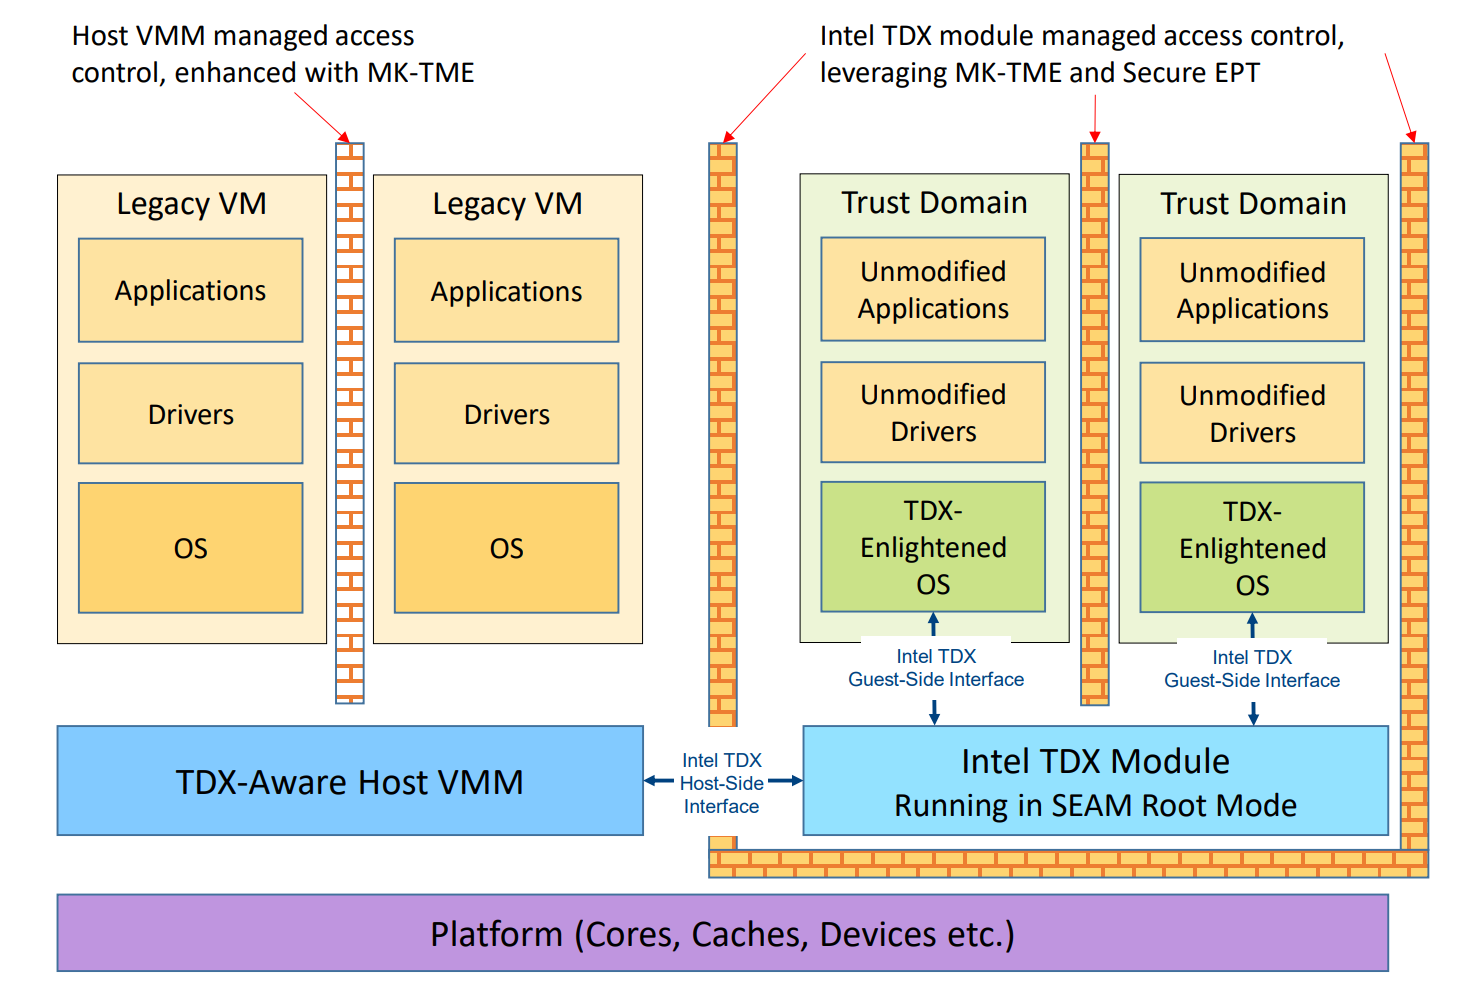
\includegraphics[width=\textwidth]{figures/TDX-Component-Overview}
\caption{TDX Component Overview taken from \cite[p.~19]{noauthor_tdx-module-10-public-specpdf_nodate}. Shown here is an extension of the Compute Stack in Fig. \ref{fig:computestack} with the colors corresponding to the non-TDX variants.}
\label{fig:component-overview}
\end{figure}
\begin{itemize}
    \item TDX-enabled processors, which offer architectural functionalities like hard-ware-assisted virtualization, memory encryption/integrity protection, and the ability to certify TEE platforms,
    \item TDX Module, an Intel-signed and CPU-attested software module that leverages the features of TDX-enabled processors to facilitate the construction, execution, and termination of TDs while enforcing the security guarantees. 
\end{itemize}
Additonally it also shows the surrounding environment containing optionally normal VMs, the hardware and TDs ontop of the TDXM.The TDX Module provides two sets of interface functions, host-side interface functions for a TDX-enlightened hypervisor and guest-side interface functions for TDs. It is loaded and executed in the SEAM RANGE, which is a portion of system memory reserved via UEFI/BIOS. The P-SEAM Loader, which also resides in the SEAM RANGE, can install and update the TDX Module. More information on the loading process can be found in \cite{noauthor_white_nodate} and \cite{noauthor_tdx-module-10-public-specpdf_nodate}. P-SEAM will be discussed further in \ref{Security Analysis}.
A TDX-enlightened hypervisor operates in the traditional VMX root mode and utilizes the SEAMCALL instruction to call host-side interface functions (function names start with TDH) of the TDX Module. Upon execution of the SEAMCALL instruction, the logical processor transitions from the VMX root mode to the SEAM VMX root mode and starts executing code within the TDX Module. Once the TDX module has completed its task, it returns to the hypervisor in VMX root mode by executing the SEAMRET instruction. On the other hand, TDs run in the SEAM VMX nonroot mode. TDs can trap into the TDX Module either through a TD exit by invoking the TDCALL instruction or triggered by some external event, e.g. an external interrupt or exception. In both cases, the logical processor transitions from the SEAM VMX nonroot mode into the SEAM VMX root mode and starts executing in the context of the TDX Module. \cref{fig:seamFigure} shows these transitions and their counter parts.

\begin{figure}
\centering
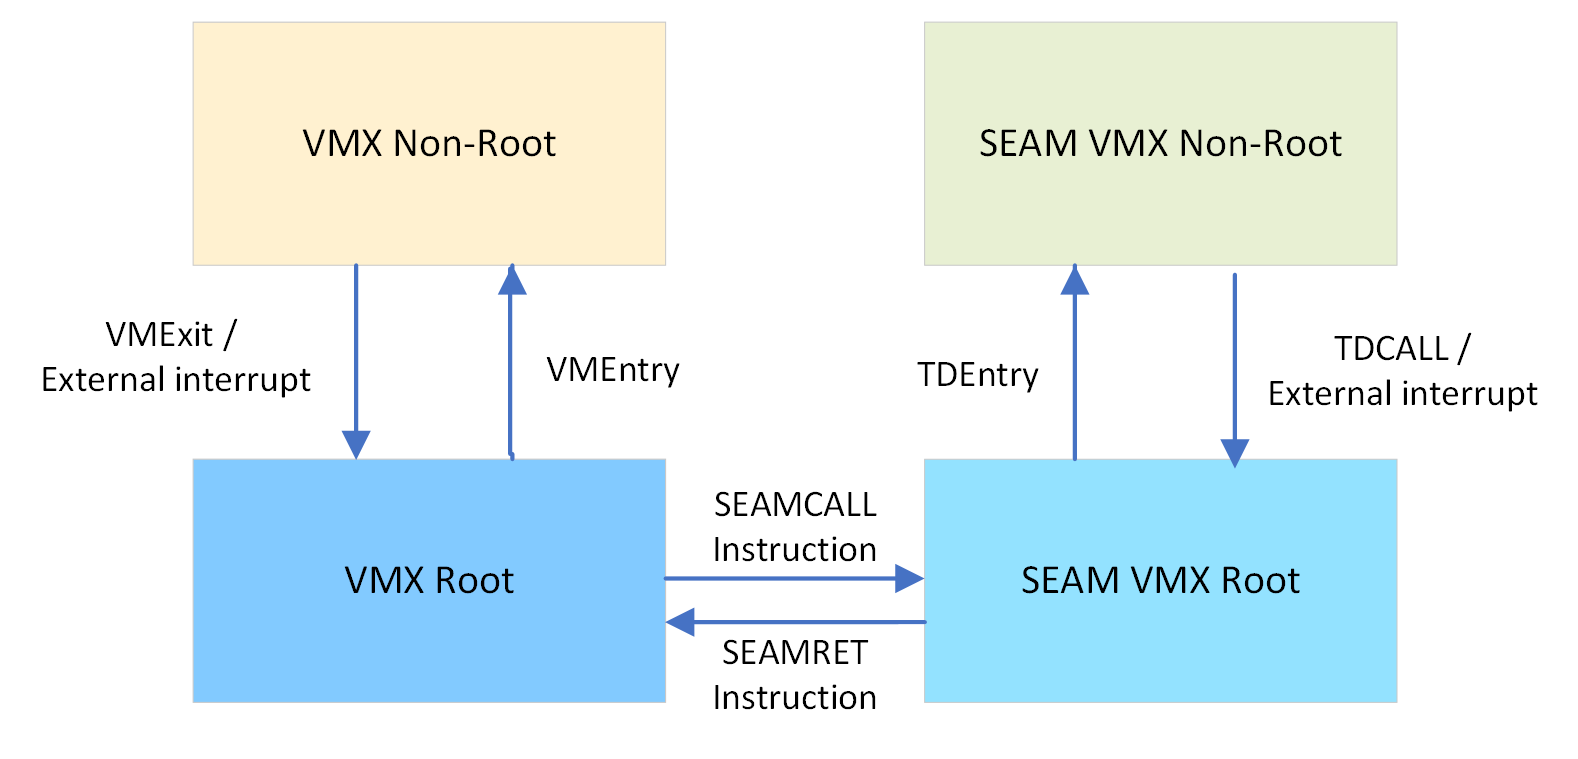
\includegraphics[width=0.7\textwidth]{figures/SEAMVMXÜBergänge.png}
\caption{VMX and SEAM VMX transitions. The colors are the same as they are for the implementations of these in \cref{fig:component-overview}. Note that it is not possible to transition from VMX non-root to SEAM non-root directly, as this would correspond to a direct transition from a TD to a non-TD vm.}
\label{fig:seamFigure}
\end{figure}
\subsection{TDX Key Generation and TD encryption}
The Host Hypervisor or Virtual Machine Manager (host VMM), which explicitly is not part of the TDX module but is aware of it calls the TDH.SYS.KEY.CONFIG function during startup, which configures the TDX modules global private key on the current CPU package \cite{intel_corporation_intel-tdx-module-15-abi-spec-348551001pdf_2024}. \todo{Was genau heißt configures private key on current package?} The host VMM can create a new guest TD by allocating and initializing a TD root control structure. The host assigns the TD a Host Key ID (HKID), which can be used to tag the memory accesses made by the TD\cite{noauthor_tdx-module-10-public-specpdf_nodate}. Subsequently, the host VMM calls the MKTME hardware, which encrypts the specified memory using a hardware-generated encryption key\cite{noauthor_multi-key-total-memory-encryption-spec-14pdf_nodate}. The VMM of the TD host configures the MKTME hardware by calling the TDH.MNG.KEY.CONFIG function on each CPU package. This will program the encryption key into the MKTME encryption engines\cite{noauthor_tdx-module-10-public-specpdf_nodate}. At this point, the TD private memory section is created and accessible by the TD. The VMM can then use Intel TDXM interface functions to create control structures. 
\subsection{TDX Attestation}
\label{TDX attestation}
Hardware attestation is a process that ensures the integrity and trustworthiness of hardware components in a computing system. It involves verifying the identity and expected behavior of hardware components connected to the motherboard. This verification is done by checking identification codes and comparing them to expected values. Attestation is necessary to establish trust for a challenger, that the used hardware is as expected. Without attestation the security assurances by TDX are not guaranteed. 
\label{Pre-Attestation setup}
Before any attestation request can be answered the platform itself must be registered. This is done by creating a shared platform key using the hardware-keys of the different CPUs on the platform. This shared platform key is then encrypted using those hardware-keys and flashed into the BIOS. After booting the host platform accesses this certificate, called platform manifest, and registers the plattform at the Intel SGX Registration service. During this registration Intel checks the validity of the platform manifest. From this platform manifest the public key of the Provisioning Certification Enclave (PCE) is then signed by Intel and returned. The Trusted Domain Quoting Enclave (TD QE) now needs to receive this signed key but it does not have a secure channel of communication with the PCE. TD QE and PCE now verify that they are on the same platform via local attestation. The AKcert in Fig. \ref{fig:local-attestation} contains the signed key. 

\begin{figure}
\centering
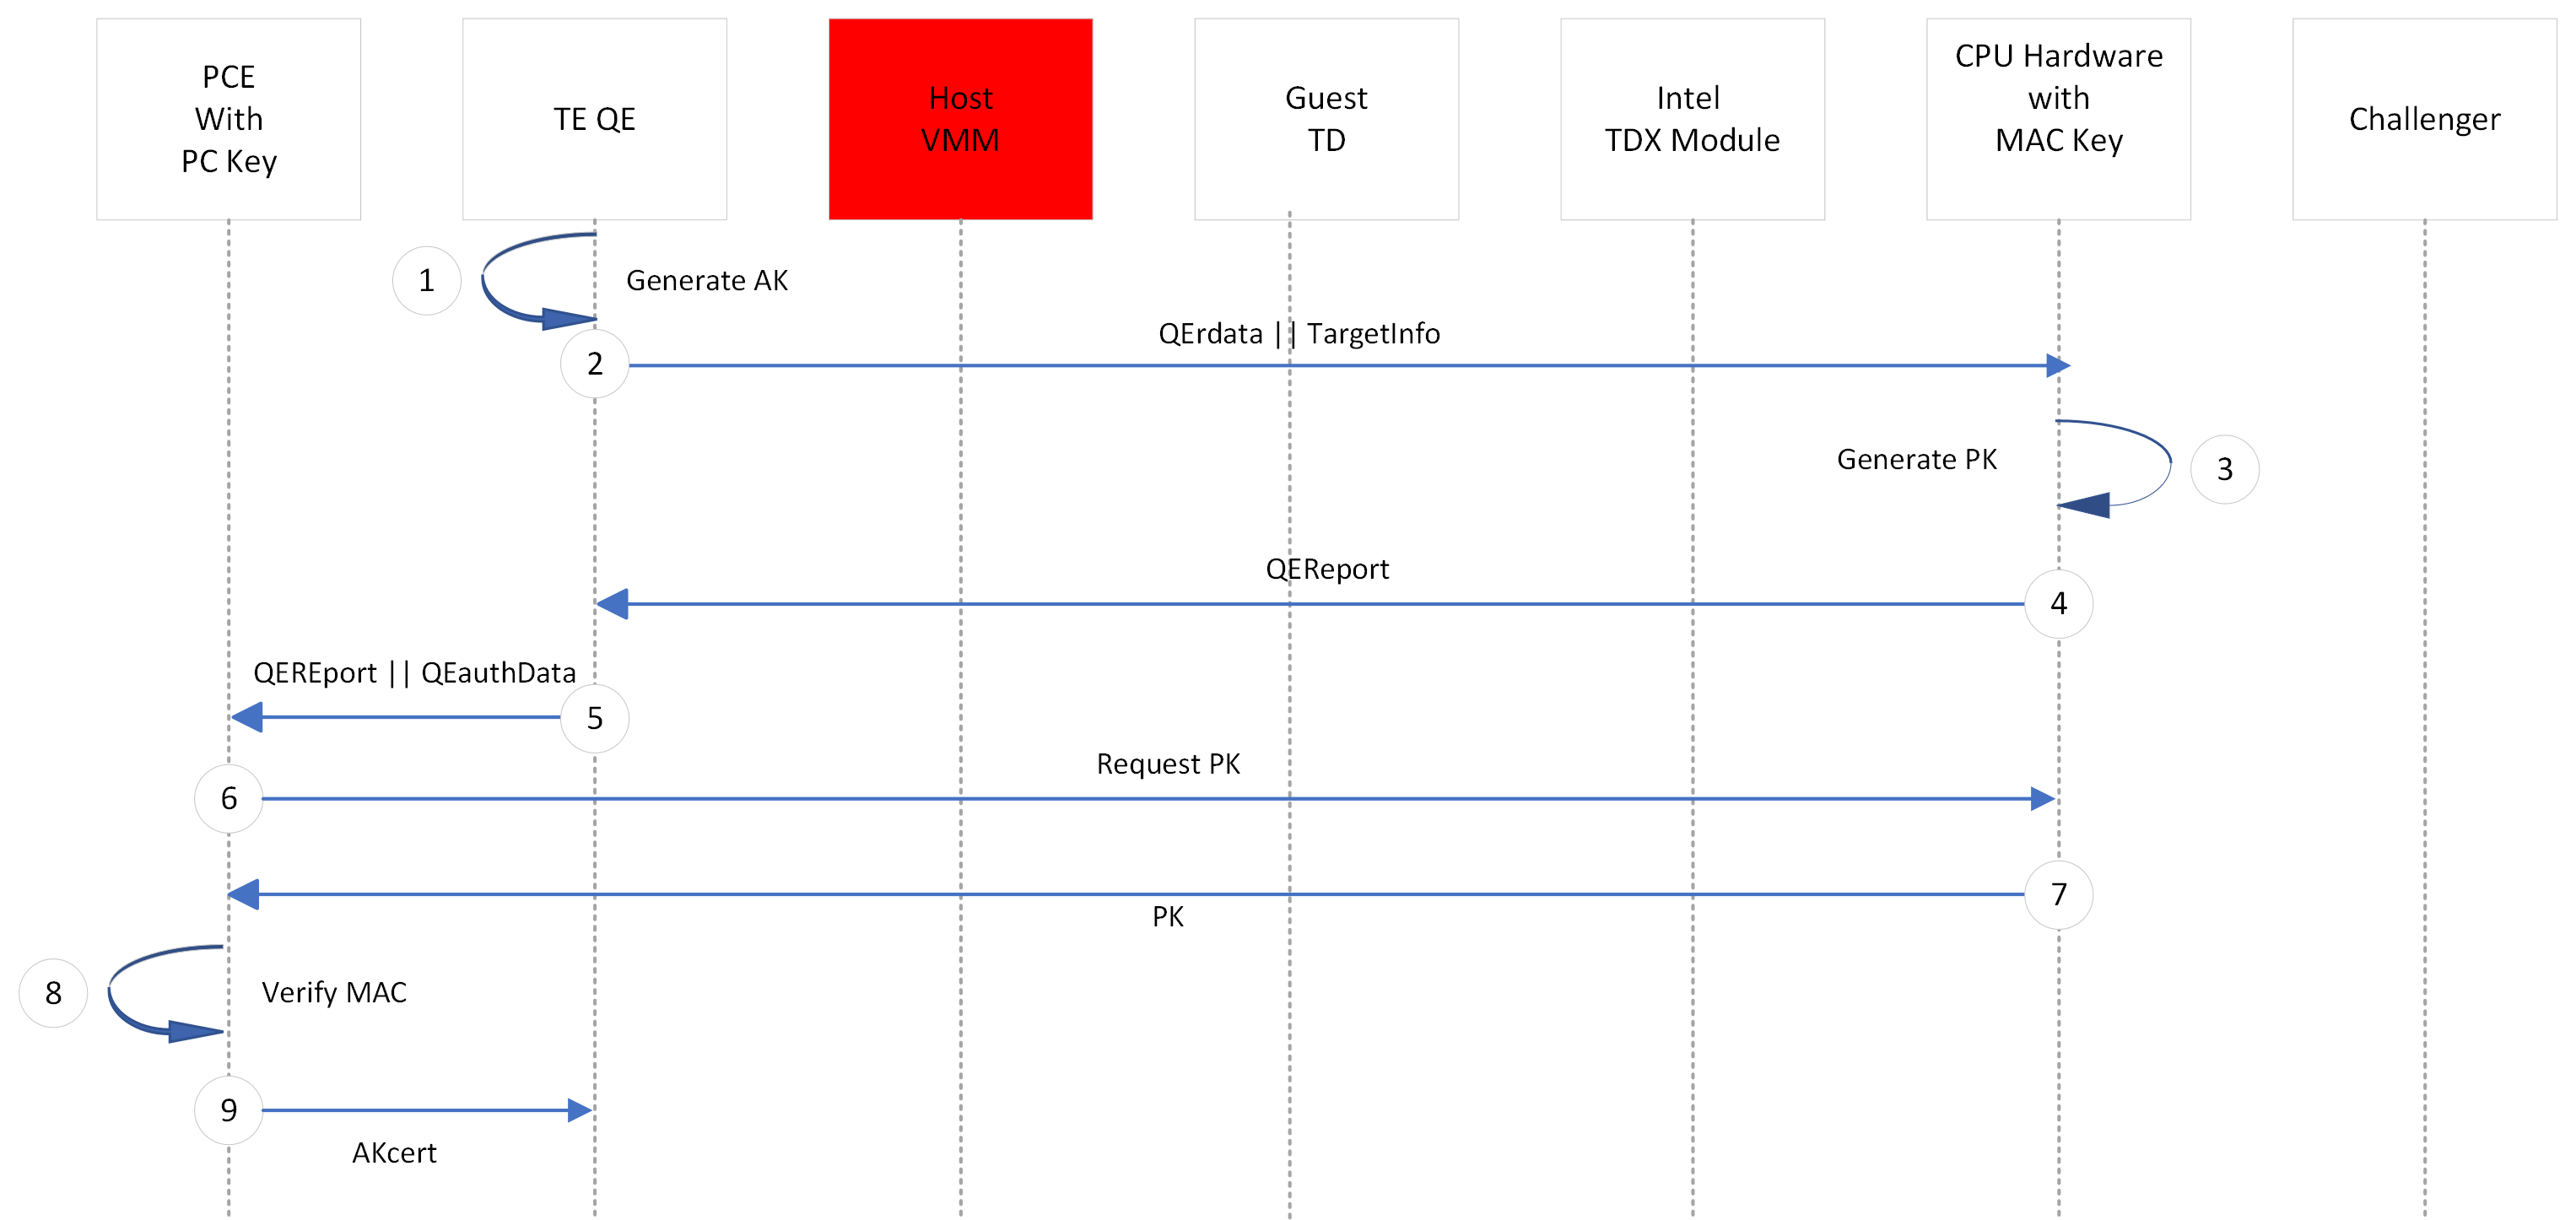
\includegraphics[width=\textwidth]{figures/Local-Attestation.png}
\caption{Intel TDX local attestation flow diagram. Text above the arrow represents data being sent, text below function calls. The Host VMM in red is untrusted. The challenger is shown to have the same entities as \cref{fig:QuoteGeneration}. Adapted from \cite{sardar_formal_2023}}
\label{fig:local-attestation}
\end{figure}

Complementary to the three provisions required by the Confidential Computing Consortium, in the context of attestation according to \cite{sardar_demystifying_2021}, the four most interesting properties are:

\label{FourProperties}
\textit{Integrity}: Claims within Evidence represent the present condition of the Attester and contain components such as identity fields. Therefore, it is crucial to prevent the adversary from altering Claims while they are being transported from the Attester to the Verifier. Typically, the integrity of Claims is safeguarded through digital signatures utilizing an Attestation Key. If the correspondence assertion holds true, it signifies that the adversary cannot modify the variables of agreement without being detected. 

\textit{Freshness}: The freshness of Evidence is crucial because otherwise an attacker has the ability to replay authentic Evidence from a previous session while simultaneously altering the state of the Attester.

\textit{Secrecy}: It must be ensured that the adversary does not have access to attestation-related keys or secrets shared between Attester and Verifier

\textit{Authentication}: The Verifier must ensure it communicates with the intended Attester. Informally, if the Verifier receives the public key of the Target Environment, this uniquely matches the public key generated within the Target Environment.

Hardware attestation establishes trust into the hardware but not the software being executed. The Attestation does however generate a quote that contains additional information on the TD and the software being executed. Trusting the Quote does not mean trust with the TD is established but only that the information in the quote is to be trusted. This establishes the environment of the TD, mainly the specific hardware and the TDX Module. With the additional information about the VM and the Image in the Quote verification might be possible but the implementation of that is left to the software developer. More information on this can be found in \ref{Identity}.
The TD attestation protocol involves six key entities: the Quoting Enclave (QE), the host Virtual Machine Manager (VMM), the guest trust domain (TD), the Intel TDX module, the CPU hardware and the challenger. The QE is an Intel-provided enclave that signs the report body after its successful verification to create a remotely verifiable Quote. The VMM is an untrusted hypervisor that manages Virtual Machines. The guest TD is an enhanced Virtual Machine that is initialized and measured at boot time. The TDX module is Intel-provided software that is signed by Intel and manages the interaction between the TD and the VMM. It is also part of the attestation metadata. The CPU hardware generates and verifies the report. Lastly, the challenger (also known as the relying party) is the remote party that performs the attestation verification.
\begin{figure}
\centering
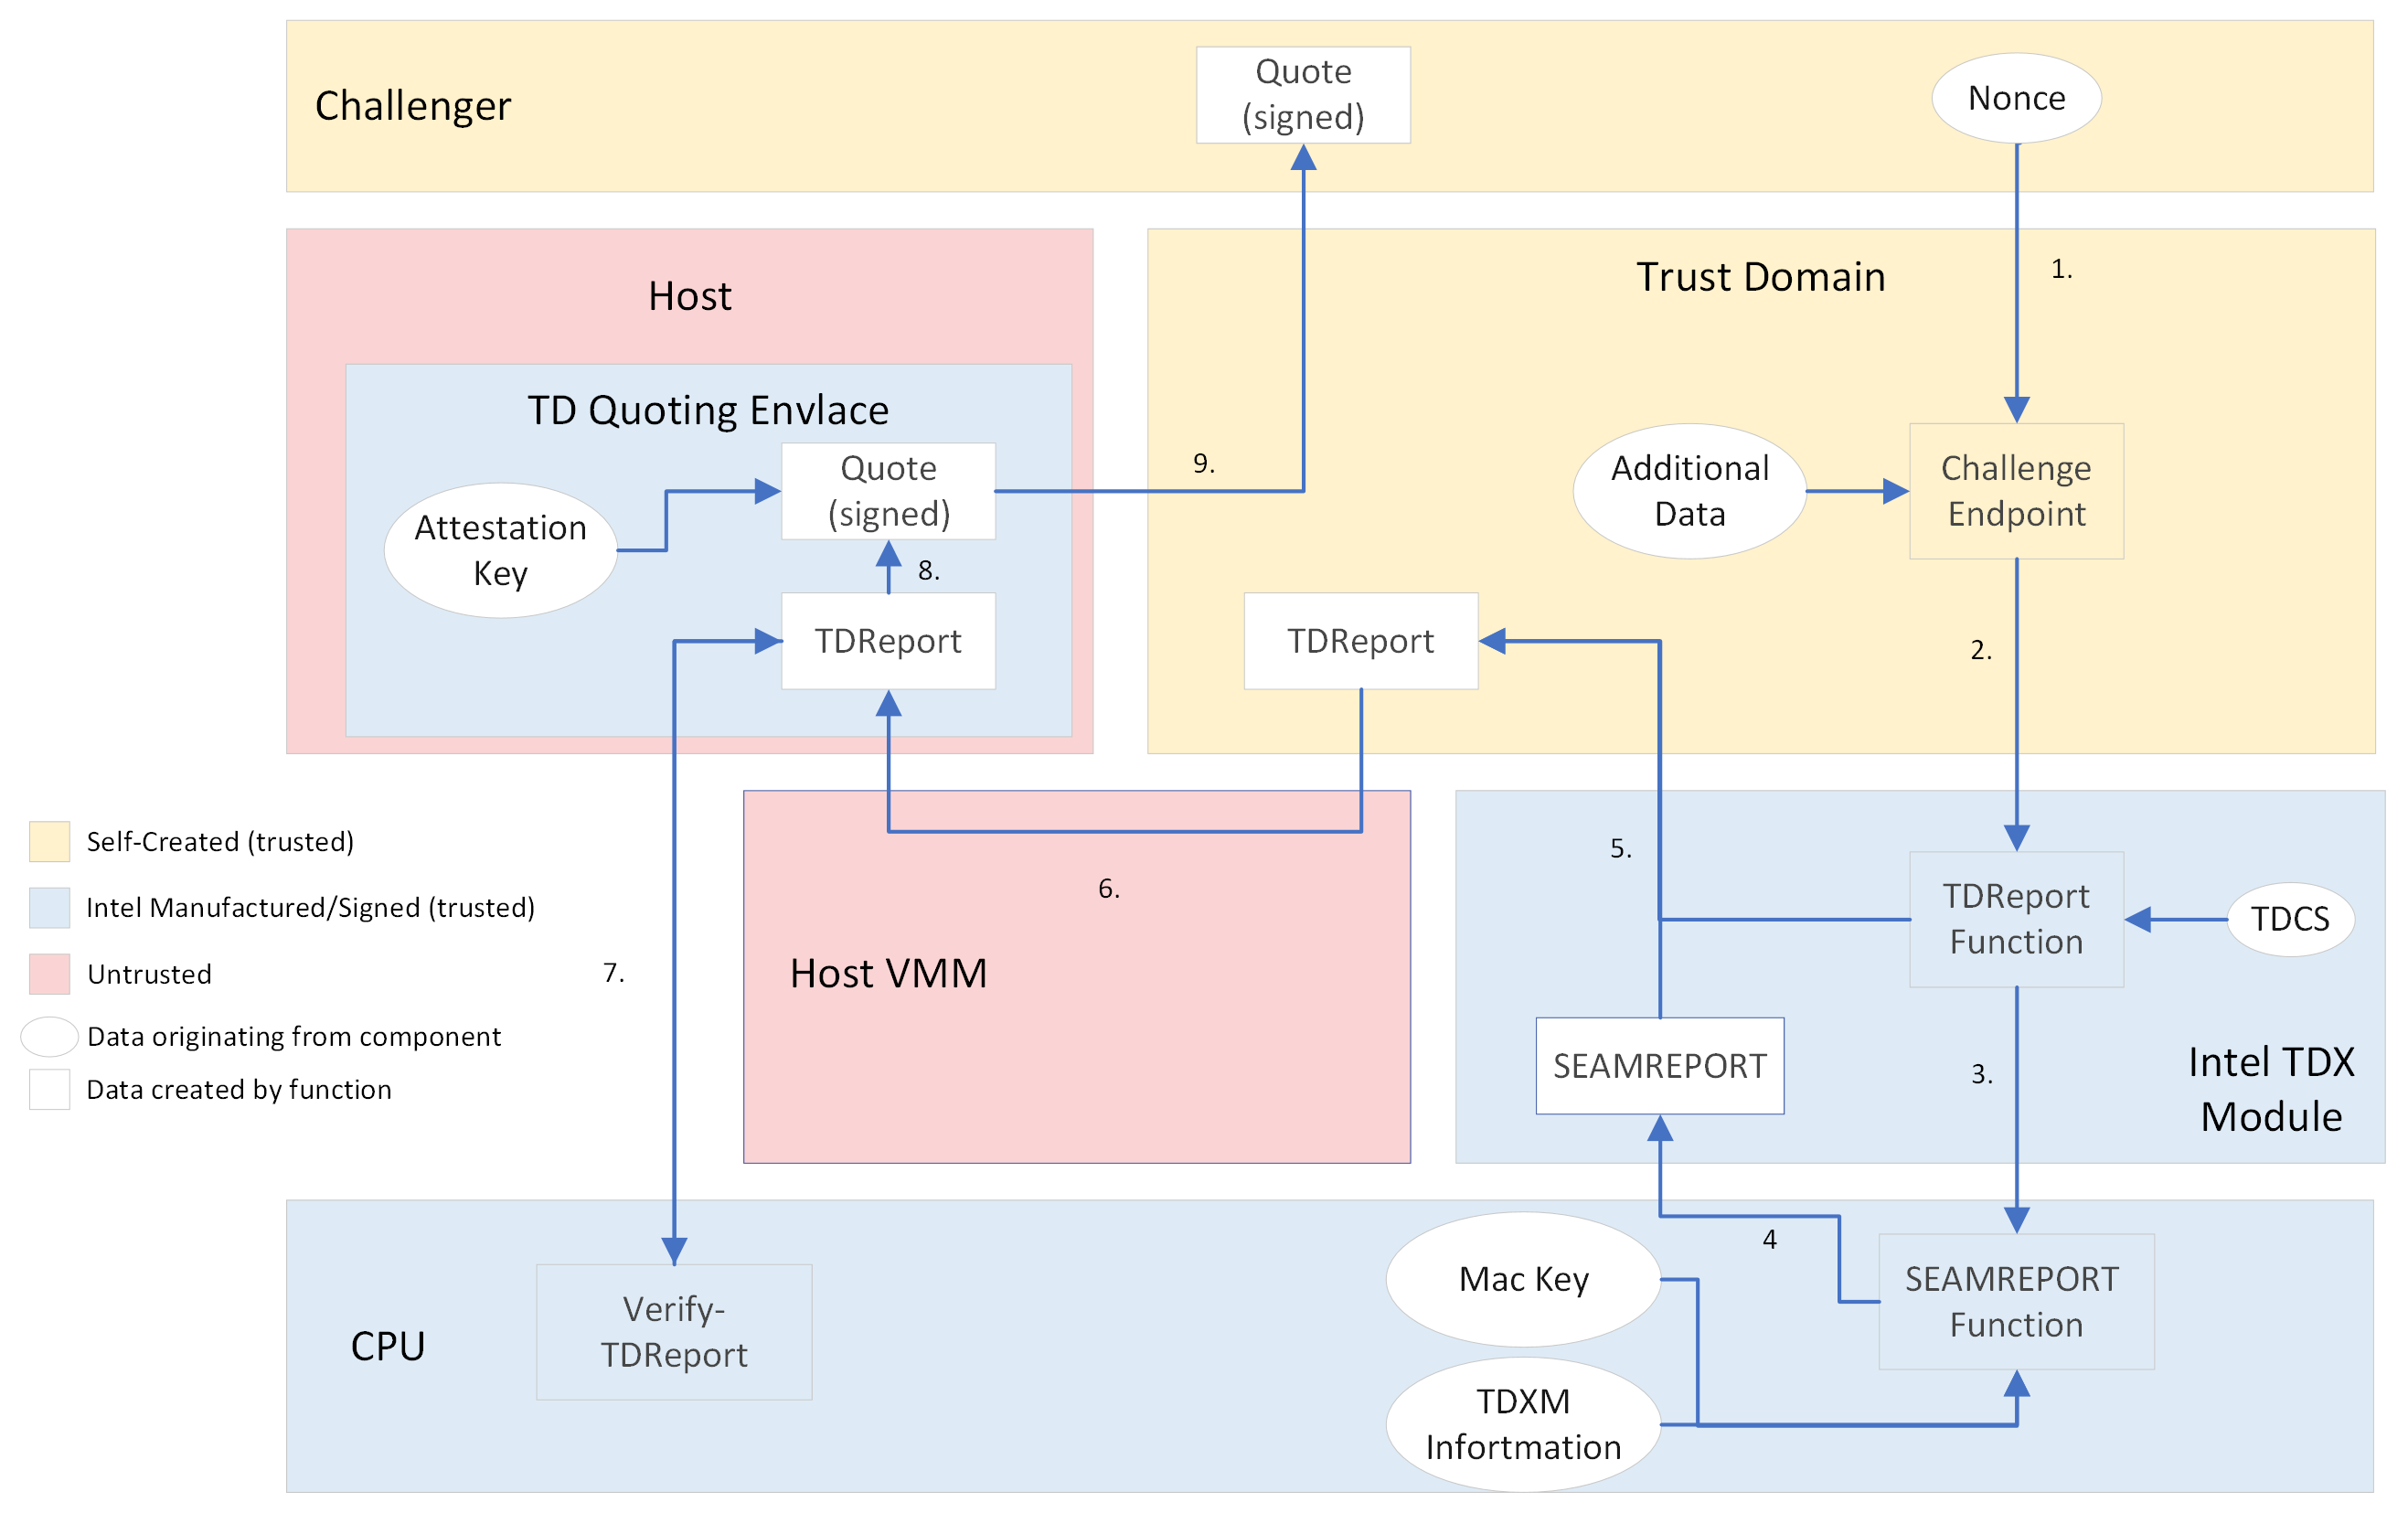
\includegraphics[width=\textwidth]{figures/Attestation-einfach.png}
\caption{A simplified SGX-based TD attestation flow. Adapted from \cite[p.~111]{noauthor_tdx-module-10-public-specpdf_nodate}}
\label{fig:EasyAttestation}
\end{figure}
Figure \ref{fig:EasyAttestation} shows a rudimentary TDX attestation flow with trusted and untrusted entities as well as their boundaries. The challenger requests a quote from the guest TD for challenge. He can include a one-time key, called nonce to prevent replay attacks. A quote is all the information necessary to attest to a specific set of hardware. After receiving the request the guest TD can supply additional runtime data, which is important to verify the authenticity of the TD, and will then send a request via a character device to the TDX module. This report contains data the TDX module holds about the TD, most importantly measurements relating to the creation of the TD, and the data that was supplied by the TD. To prevent issues with the data transfer via the untrusted Host VMM the CPU has a Message Authentication Key (MAC) from the TD QE, which it uses to encrypt the TDReport. The TD QE now calls the CPU again to verify the integrity of the TDReport.
To create a chain of trust, which can only be accessed via Intel, the Attestation key was previously signed by the PCE key, which was signed by Intel. This means that the Quote can in the end only be decrypted via an Intel service.

\begin{figure}
\centering
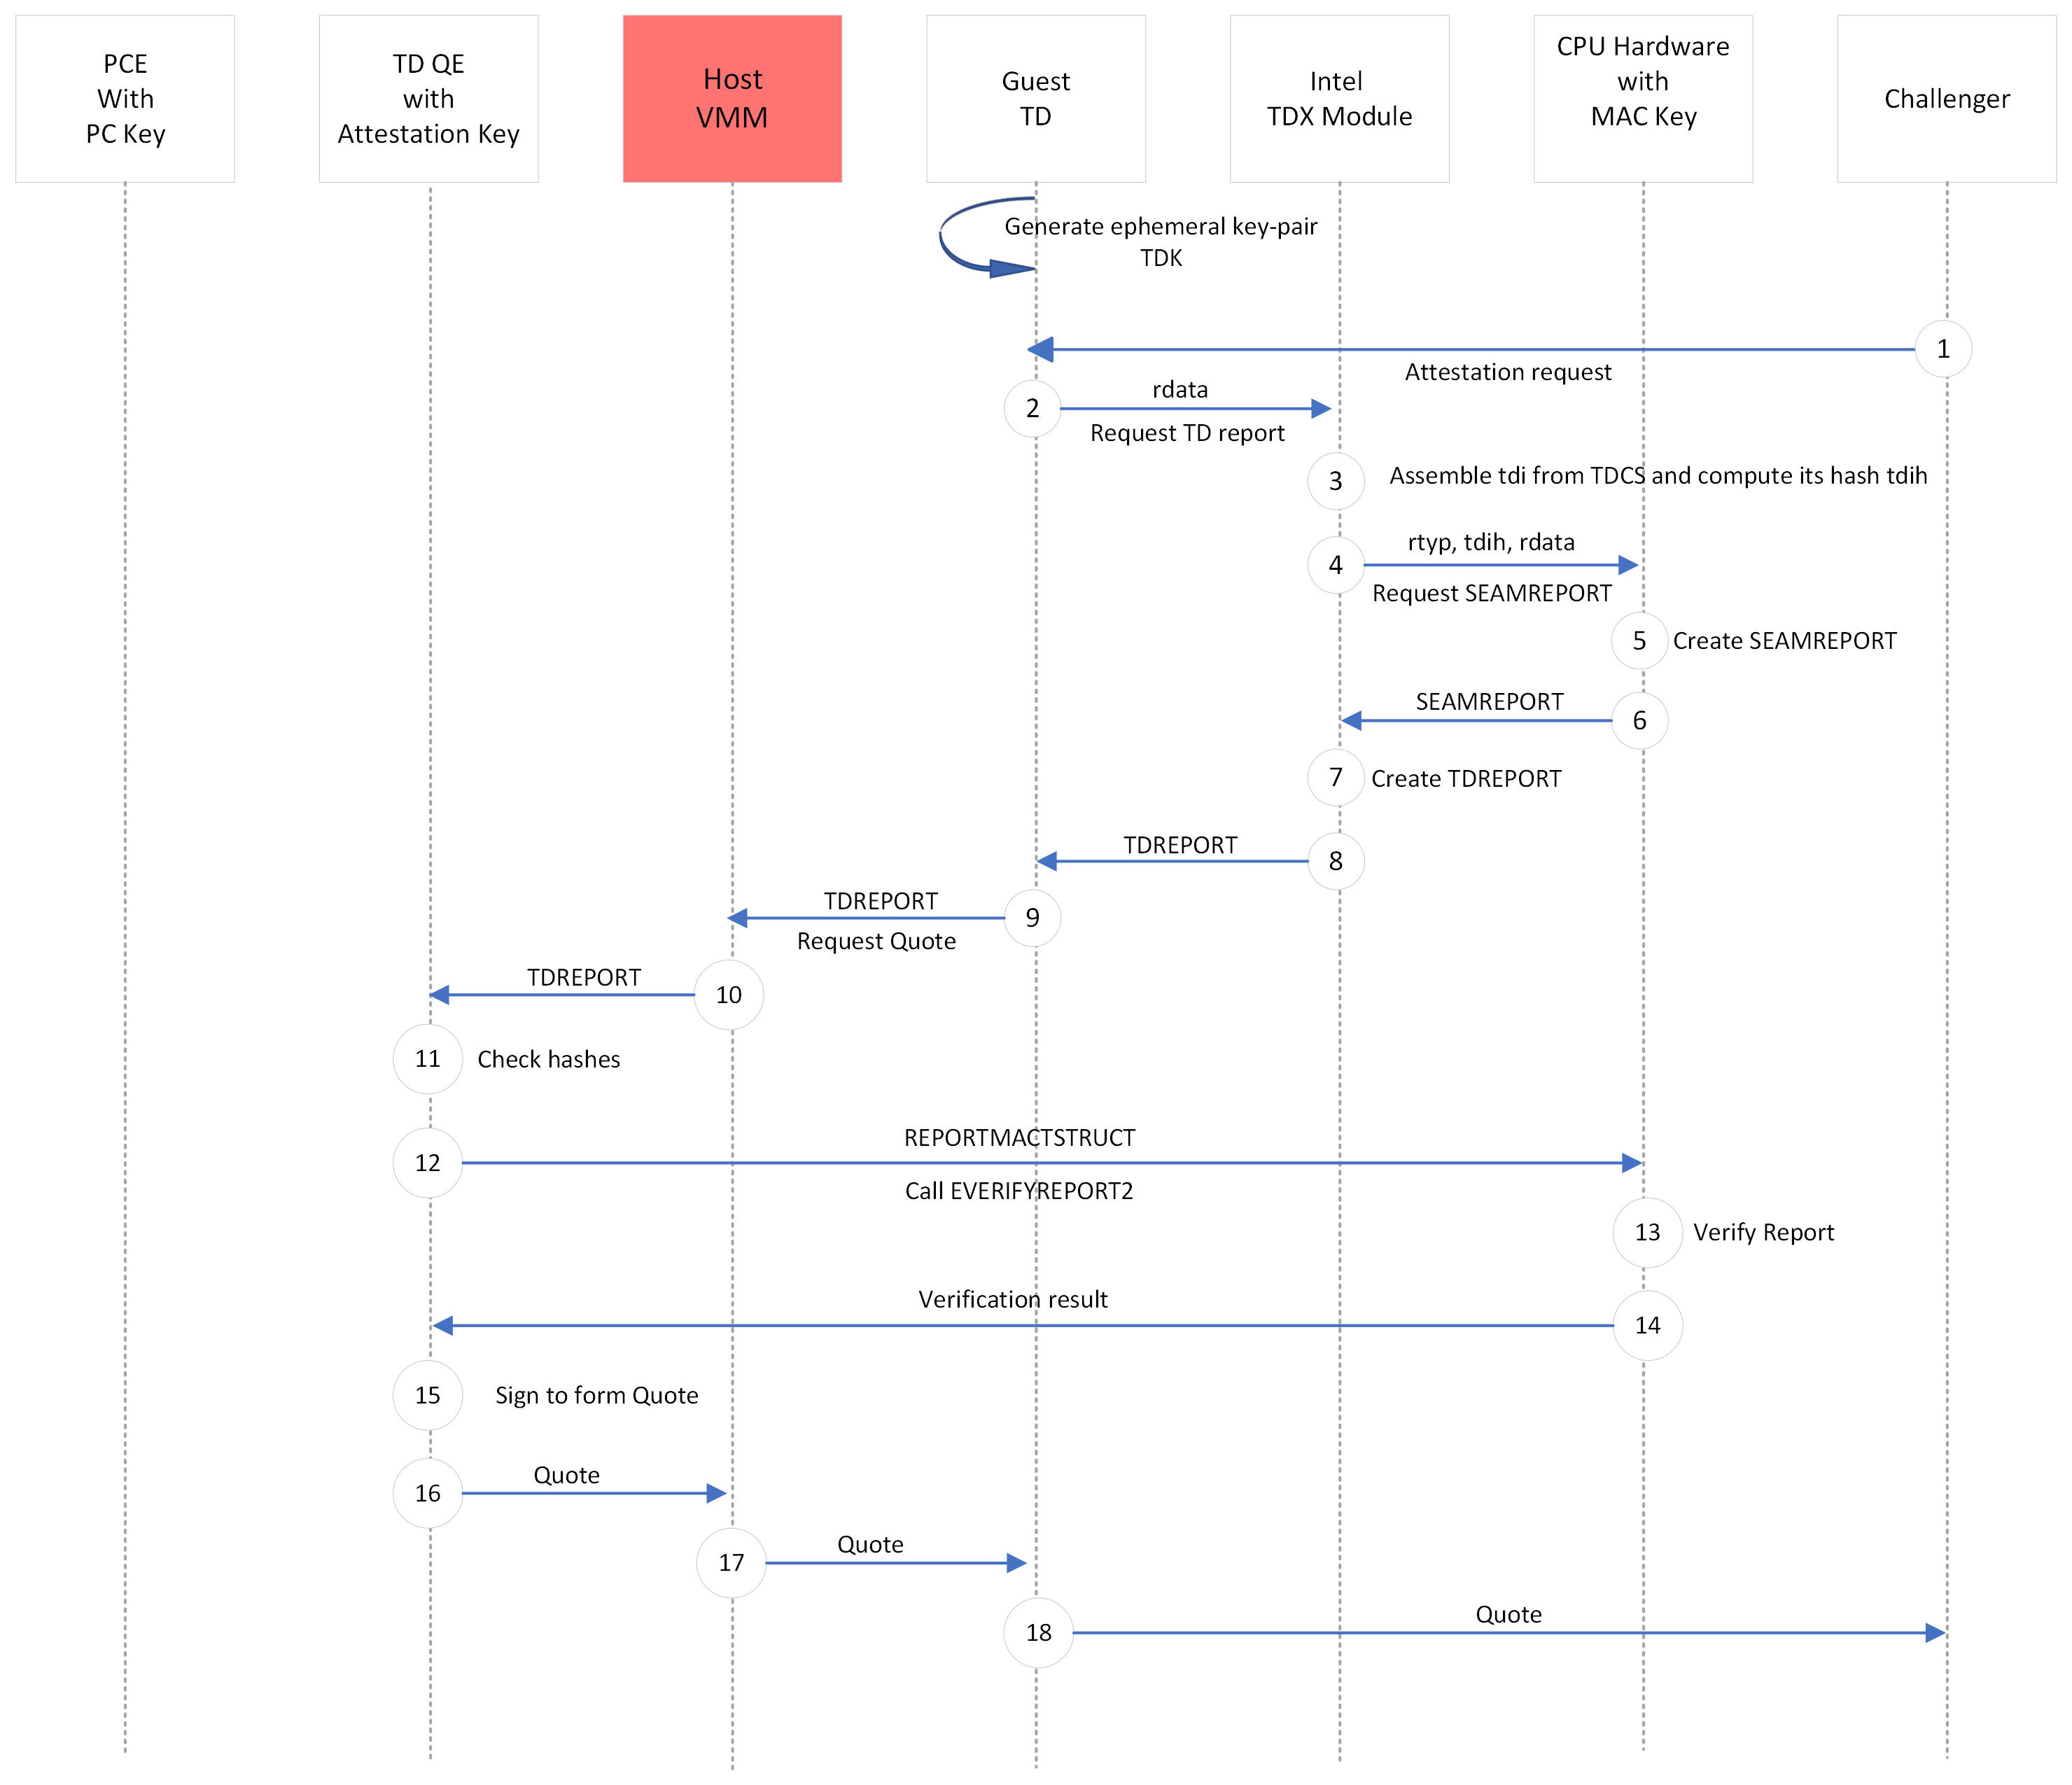
\includegraphics[width=\textwidth]{figures/Attestation Diagram.png}
\caption{Intel TDX Attestation flow diagram. Text above the arrow represents data being sent, text below function calls. The Host VMM in red is untrusted. The PCE is shown to have the same layout as \cref{fig:pre-attestation}. Adapted from \cite{sardar_demystifying_2021}}.
\label{fig:QuoteGeneration}
\end{figure}
The following will now explain each step in more technical detail, while using Figure \ref{fig:QuoteGeneration} as reference. 
TDX includes a set of major functions explained here. \textit{Sign} represents the Elliptic Curve Digital Signature Algorithm signature over the message with the specified signature key. 
Calculating the \textit{hash} means computing the SHA384 of the input. \textit{Hmac} is HMAC\_SHA256 of the message with the specified key. More information on hmac can be found in \cite{hmac_keying_1996}. The message is not extractable if hmac is considered a pseudorandom function, which in practice appears to be true\cite{bellare_new_2006}. The TDK key-pair is sometimes also called TD key-pair.
\newcommand\setItemnumber[1]{\setcounter{enumi}{\numexpr#1-1\relax}}
\begin{enumerate}
\item The challenger initiates the attestation process by sending a challenge request to the Guest TD. This can include a nonce to prevent replay attacks\cite{sardar_formal_2023}.
\item TD calls TDG.MR.REPORT by sending the hash of the TDK public key and the challenge to the TDXM (using rdata). On Linux this can be done via the character device tdx\_guest. This triggers a TDExit as shown in \cref{fig:seamFigure}
\item TDXM assembles TD information data structure tdi from Trust Domain Control Structure (TCDS) and computes its SHA384 hash tdih. The TCDS contains the following information:
\begin{itemize}
    \item Fields designed to control the TD operation as a whole (e.g., a counter of the number of VCPUs currently running). 
    \item Fields designed to control the execution control of the TD (debugability, CPU features available to the TD, etc.). 
    \item Registers filled with static and runtime measurements. 
    \item EPTP: as designed, a pointer (HPA) to the TD’s secure Extended Page Table (EPT) root page and EPT attributes
    \item Model Specific Register (MSR) bitmaps, designed to be used by all the TD’s VCPUs. 
    \item A page filled with zeros, designed to be used in cases where the Intel TDX Module needs a read-only constant 0 page encrypted with the TD’s private key.
\end{itemize}
\item TDXM calls SEAMOPS[SEAMREPORT] with tdih and rdata
\item[5. \& 6.] CPU generates SEAMREPORT smr  with rms (red) and tcbi (purple) \ref{fig:tdr} and returns it to the TDX module. This importantly contains measurements about the TDX module and about the TDX module signer, in this case Intel.
\setItemnumber{7}
\item TDXM builds tdr with smr, res4, and tdi. Content for the entire tdr can be seen in Figure \ref{fig:tdr}
\begin{figure}
\centering
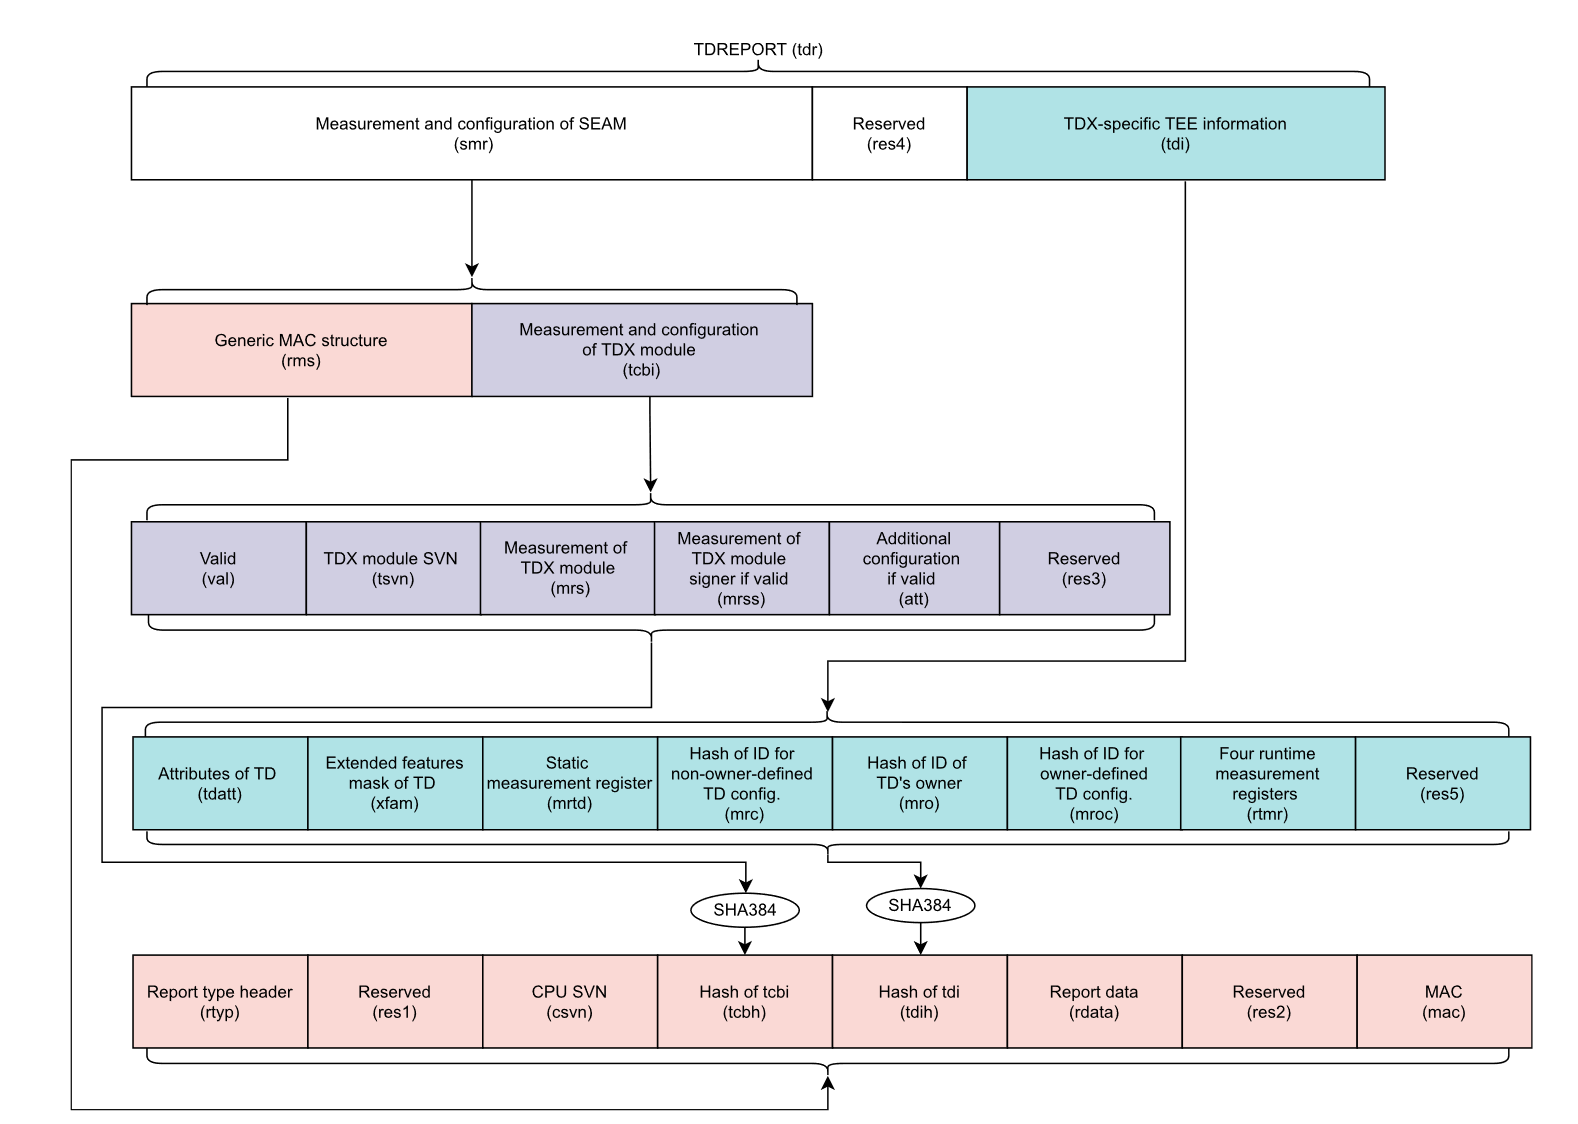
\includegraphics[width=\textwidth]{figures/tdr.png}
\caption{An overview of the component of the TDREPORT taken from \cite{sardar_demystifying_2021}}
\label{fig:tdr}
\end{figure}
\item TDXM sends tdr to the Guest TD
\item[9 \& 10.]The Guest TD sends tdr to the TD Quoting enclave, via the untrusted VMM
\setItemnumber{11}
\item TD QE verifies the hashes in report
\item Rms (part of smr, red in Fig \ref{fig:tdr}) is used as an argument in the ENCLU[EVERIFYREPORT2] cpu function. 
\item[13. \& 14.] CPU performs the verification of rms and returns the result to the TD QE. The verification consists of three main steps: 
\begin{enumerate}
\item verify that the header rtyp in the report is correct, 
\item verify that the CPUSVN csvn is a valid value, and 
\item compute the MAC over the fields in the report body rptbody using the MAC key MACkey, and verify that the computed MAC matches the value in the field mac of the received report (represented as receivedMAC)
\end{enumerate}
\setItemnumber{15}
\item TD QE replaces the MAC with a Quote defined as <rptbody, (sign(AK, rptbody))>.
\item[18. \& 19.] Quote is sent to TD, VMM is untrusted → Sent by public channel
\setItemnumber{18}
\item TD sends quote to relying party(RP)
\end{enumerate}
The challenger can now verify the Signature on the Quotebody by going back the chain of trust rooted at Intel. This verification is based on the Data Center Attestation Primitives (DCAP) which will be explored later on in \ref{Security Analysis}. After verification the challenger can now send a secret encrypted with the public key of the TD to the TD establishing a common secret for further secure communication. If the TD did not include a public key in its quote section \ref{Establishing_a_secure_connection} contains further information on how to establish a secure connection. According to \cite{sardar_formal_2023} using ProVerif, this ensures integrity for the tcbi, tdi and rdata. It also ensures freshness and secrecy. Authentication does not hold as long as secure communication via TLS or similar is not established.

\section{Related Work}
TDX has been looked at a fair amount of times already. In particular, a nearly complete security analysis of its hardware and the low-level TDX software by Aktas et al. at Google \cite{aktas_intel_nodate}. They limited their analysis to just the host-side without looking at TD user or developer issues down the line. Similarly, Sardar et al. formally verified TDX attestation in \cite{sardar_demystifying_2021}. They looked at the theoretical security of a perfect implementation. Knauth et al. introduced a way to create a secure channel using Intel SGX \cite{knauth_integrating_2019}, this will be used as the basis to establishing a secure channel to the TD in this thesis. Cheng et al. briefly mention this as well, but their focus was more generally on the TDX architecture \cite{cheng_intel_2023}. This thesis explores the feasibility of those for an average user, as well as its security assumptions and pitfalls. Lefeuvre et al. have looked at difficulties and issues with safe and confidential I/O \cite{lefeuvre_towards_2023}, this will only be briefly touched upon in this thesis. Delignat-Lavaud et al. looked at issues pertaining the TCB of confidential services. Their information was used in this thesis to look at the feasibility of using CC for the average user. Their consensus was picked up in this thesis that while CC is great in theory, the practice is lacking.



\chapter{Methodology}

- Mad vs std dev
- Performance testing how to
- How to rank values / Zangenmeister?

%% LaTeX2e class for student theses
%% sections/content.tex
%% 
%% Karlsruhe Institute of Technology
%% Institute for Program Structures and Data Organization
%% Chair for Software Design and Quality (SDQ)
%%
%% Dr.-Ing. Erik Burger
%% burger@kit.edu
%%
%% Version 1.4, 2023-06-19

\chapter{Security Analysis}
\label{Security Analysis}

This chapter contains an overview of threats and how, if so, \Gls{TDX} protects against them. This analysis is by no means comprehensive, but meant as an overview. It gives examples of real attacks using the aforementioned attack vectors. In addition ways to establish a secure connection to a TD and TD identity verification are discussed.

\section{Already known attacks and vulnerabilities}

This section gives examples of attacks inside and outside the threat model that have already been proven to be effective against either \Gls{SGX} or TDX. The line what is inside the Threat model and what is outside can sometimes be vague, especially in regards to physical attacks. In \cref{Threat_Model} I have already tried to clear this up and this section will explain some attacks that can break TDX.

As described in \cref{Threat_Model} TDX considers the cloud provider, with physical access, as untrusted. This means that any physical attack should be defended against, but as outlined previously this is not the case. Opening the case does not provide a significant hurdle for any attacker, who already has physical access. This leaves TDX vulnerable to any sort of attack that can be executed with physical hardware access, that can break \Gls{SGX}. This includes Plundervolt which can break the integrity and indirectly the confidentiality of \Gls{SGX} \cite{munoz_survey_2023}, which is, as outlined in \cref{TDX Architecture} relied upon for TDX. Platypus attack which was also shown to break the integrity of \Gls{SGX} \cite{Lipp2021Platypus} and more \cite{lipp_nethammer_2018} \cite{tang_clkscrew_nodate}. While attacking a specific TD inside a data center is non-trivial it is not impossible. This means that as long as hardware access is not prevented completely TDX can not prevent access to data inside the TD. TDX can by their very nature not protect against all side-channel attacks. It protects against some well known ones such as the spectre-family. TDX does not have mitigations to address memory access patterns as it just uses encrypted memory. Privacy leakage from memory access attacks was already shown to take less than a couple of minutes on consumer grade hardware. John et Al. were able to infer a 512-bit secret in just three and a half minutes only using write-access patterns \cite{john_connecting_2017}. 



\section{Connecting to the correct TD}

This section explains how to verify a TDs identity and then how to securely connect to this TD. Without verifying the TDs identity a secure connection can not be established, because the endpoint is not verified.

\myparagraph{Verifying the TD identity}

\label{Identity}
Similarly to \Gls{SGX}, with \Gls{TDX} the quote contains information on the startup environment of the TD. The Measurement of Trust Domain (MRTD) registers contain information on the initial state of the TD immediately after startup. Its calculation is based on the page content during startup \cite{intel_corporation_dcap_2024-1}. The Runtime Measurement Registers (RTMR) are written during runtime, Intel recommends writing information about the virtual firmware configuration in RTMR[0] and information about the OS kernel and boot parameters or more importantly kernel parameters in RTMR[1]. Information about these can be supplied by the virtual firmware, which is written by Intel and should thus follow their own recommendations. It is unclear when these are written. They are either filled after startup by the TDVF \cite{intel_corporation_tdx-virtual-firmware-design-guide-rev-004-20231206pdf_2023}, somehow supplied by the host, although this would make them untrusted and worthless, written after the TD requests the TDX Module to do so \cite{intel_corporation_tdx-virtual-firmware-design-guide-rev-004-20231206pdf_2023} or just filled by the TD itself \cite{noauthor_tdx-module-10-public-specpdf_nodate}. Testing later shows that they are empty immediately after startup on an Azure VM.
RTMR[2] is used as a replacement for the Platform Configuration Register from TPM, to hold the aggregate integrity value of the IMA runtime measurement list. To do this Intel had to introduce an additional kernel driver and an update for IMA \cite{haidong_xia_runtime_integrity_measurement_2024}. The IMA update has not been made public on the official IMA repository at \url{https://sourceforge.net/projects/linux-ima/} as of yet. In the future Intel wants to support a virtualized version of TPM, so that an unaltered Kernel can be used. To ensure traceability the event logs related to the list of measurements will be kept in the Confidential Computing Event Log (CCEL) table \cite{haidong_xia_runtime_integrity_measurement_2024}. The CCEL is created during startup and rooted inside the UEFI reserved memory. The User can use either /dev/mem or /sys/firmware/acpi/tables/data/CCEL, which is read-only, to access the data inside it. Many systems have /dev/mem disabled for security reason, that is why the additional firmware table was added.

\subsection{Establishing a secure connection to the TD}

This section proposes three different ways to establish a secure connection. They are sorted in order of increasing complexity.

\label{Establishing_a_secure_connection}

\myparagraph{Simple SSH connection to a TD}

\label{SSHConnection}
Prior to TD creation the image can be build containing a known user public ssh key. If it is the only key present and password authentication is deactivated, the TD will decline connection attempts by anyone without the corresponding private key. This is generally how cloud providers provide VMs. This being the only key present can be verified via measurements in the TD Quote as discussed previously. If possible the startup measurements should be compared to a selfbuild image containing just the users public key, if not possible the TD identity can not be verified and no secure connection can be established. The TD has to put its own public key into the REPORTDATA field of its quote so the user can then verify its fingerprint when establishing a connection. This connection is vulnerable during the first connection as it is unsecured. No sensitive data should thus be transmitted before the quote is not received and verified. After verifying the TD identity and getting its public SSH key, a new connection has to be established. If the user is the only person being able to access this specific TD then this means that it is no longer possible to fake the man-in-the-middle attack in Figure \ref{fig:man_in_the_middle} because the attacker would not have access to a TD that can create the correct quote. This form of secure communication relies on the fact that only one public key is in the TD. It also depends on the user to verify the TDs identity upon connecting and also for subsequent connection attempts that the fingerprint of the TDs cannot be recreated for transcript collision attacks \cite{bhargavan_transcript_2016}.

\myparagraph{TLS connection to a TD}

According to Cheng et Al. \Gls{TDX} and \Gls{SGX} can establish secure channels via TLS in a similar way \cite{cheng_intel_2023}:
In a typical scenario, when a client negotiates a secure channel with a server running in a TD, it aims to ensure a connection with a server that has been properly instantiated. The server, acting as an attester, generates a pair of ephemeral public and private keys. It calculates the hash of the public key, creates a TD quote with its key inside the REPORTDATA and generates a self-signed certificate with the quote embedded in it. This self-signed certificate is provided as the server certificate in the TLS handshake protocol. Upon receiving the server certificate, the client, acting as the challenger, verifies the signatures on the certificate and validates the embedded quote, including the measurements. The client also checks if the quote includes the hash of the public key, as this associates the key with the TD. This contains the assumption that the client can verify the TD identity from the Quote, which is not given. When establishing a secure channel, both the client and server can assume the roles of attester and verifier. This enables endpoints running in TDs to authenticate each other mutually by validating TDs. Issues arising from self-signed certificates, the certificate size and similar are all discussed as well by Knauth et Al., with all of them having solutions \cite{knauth_integrating_2019}. Although the latter can mean that the entire TD can be compromised which invalidates other security assumptions. Therefore this variant and the SSH connection have similar security assumptions and guarantees.
Lastly an add-on to the previous method of establishing a secure connection is the usage of a complete application in the image, that does only expose certain endpoints to the web. Using proper authorisation against those endpoints, makes unwarranted access impossible. Additionally, having the application immediately on startup create the necessary certificate from the previous paragraph, prevents attacks on the initial connection as well. This is Intels recommended way of using \Gls{TDX} and starting a TD. 

\myparagraph{Using Initramfs and encrypted disk images}

Using a custom Kernel with a custom Initramfs that mounts an encrypted disk and contains \Gls{TDX} attestation capabilities as well as a predetermined public user SSH key, it is possible to establish a secure connection as well. Intel recommends implementing these capabilities in their Guest to Hypervisor communication Interface specifications aswell \cite{intel_corporation_guest_hypervisor}. This relies on the same mechanisms as \ref{SSHConnection} but gives the additional benefit, of containing an encrypted storage volume. It can thus safeguard sensitive data inside the image from unauthorized access. Upon startup the TD will pause the start after the Kernel has been loaded. The Initramfs will be loaded and active here as well. The challenger can now use its private key to the public ssh key inside the Initramfs to establish a secure connection. The challenger can now create a TD quote containing the Kernel measurements. Verifying the kernel measurements inside the TD quote and can then supply the key to the encrypted disk image to continue booting. According to Intel it should be possible to safe the encryption key inside the memory using the Storage-Volume-Key-Location ACPI Table \cite{intel_corporation_guest_hypervisor}. Intel even recommends usage of these tables in their design guide \cite{intel_corporation_guest_hypervisor}. They do not explain how these could be adequately protected from unauthorized access by, for example, the cloud provider. If disk encryption is used, dm-crypt provides the ability to use disk encryption with authentication. It is now guaranteed that the image inside the encrypted disk image is now executed only once and is running inside a TD. Choosing a secure channel to this TD depends on the code inside. Having an additional SSH key inside, as explained previously, can work.

\section{Attestation Verification}

There are generally four ways how attestation can be done that have their pros and cons. They are outlined in \cref{tab:AttestationVerification}. Intel is considered an independent vendor in this comparison as they are independent from the cloud provider that is in question. Intel is also already a trusted party, at least in terms of their hardware, and more importantly all attestation verification services have to at least talk to Intels provisioning certification service.

\begin{table}
\centering
\resizebox{0.9\textwidth}{!}{%
\begin{tabular}{ m{0.3\textwidth} m{0.2\textwidth} m{0.2\textwidth} m{0.2\textwidth} m{0.2\textwidth}}
\toprule
& Cloud Provider Attestation Service & Application Vendor Attestation Service & Third Party Trust Service (E.g. Intel Trust Authority) & Build-Your-Own Service with DCAP \\
\midrule
Seperation of responsibilities between verifier and infrastructure provider & No & Yes & Yes & Yes \\
\midrule
Consistency across SGX and TDX & Yes, if both are offered & Yes, if both are supported & Yes & Yes \\
\midrule
Consistent service across on-prem, hybrid, multi-cloud, and edge deployments & No & Possible but unlikely or limited & Yes & Yes\\
\midrule
Development Effort & Low & Low & Low & Medium \\
\bottomrule
\end{tabular}
}
\caption{Overview of four different Attestation Verification methods}
\label{tab:AttestationVerification}
\end{table}
This thesis will focus on Cloud Provider Attestation Service, and more specifically Microsoft Azure Attesation (MAA). The security assumptions and guarantees for this will then be compared to a Build-Your-Own Service using DCAP. MAA also has to use Intels DCAP to generate and verify quotes. 

\subsection{Cloud Provider Attestation Service}
 Microsoft, offers an attestation verification service hosted and implemented by them. They also offer an implementation of Intel DCAP to generate a quote. This can then be automatically verified via MAA or Intel Trust Authority or manually using your own DCAP implementation. Intel Trust Authority was not available for testing.

\myparagraph{Microsoft Azure Attestation}

This section will explain in detail how MAA can be used, the pitfalls for the user, and any other issues with it that were found. First to use MAA, one has to create a confidential VM with Azure. Microsoft provides a tutorial to create a TD VM \cite{chasecrum_github_create_2024}, which does not create a TD, that has the characteristics discussed in \cref{TDX Architecture}. The Issues with the TD used as well as the firmware are explored at the end of this section. Following the instructions provided by Azure, it is also not explained how to choose between AMD SEV-SNP and Intel \Gls{TDX}. This decision is entirely up to the chosen VM size which can only be inferred by looking at press releases pertaining to Intel \Gls{TDX} and the newly released VM sizes. The DC\textbf{e}sv5, DC\textbf{e}dsv5 and EC\textbf{e}sv5, EC\textbf{e}dsv5 use Intel Xeon CPUs, while DC\textbf{a}sv5, DC\textbf{a}dsv5 and EC\textbf{a}sv5, EC\textbf{a}dsv5 use AMD Threadripper CPUs. The difference between D-instances and E-instances is the ratio between VCPU cores and memory, with E-instances having more memory per core. With the VM created there are a couple of ways to create a TD Quote for attestation: Using an Intel-supplied or a self-written implementation of Intel DCAP and the Azure confidential-computing-cvm-guest-attestation library \cite{microsoft_corporation_azureconfidential-computing-cvm-guest-attestation_nodate}. Building the tdx-attestation app and using the supplied maa\_config file, which does only contain three settings, succeeds in creating a TD quote and then returns a JSON Web Token from the Microsoft Azure attestation Service. A complete example token can be found in \cref{jwt} but here we will focus on some parts of the td quote body. Intel has already given short explanations for all \Gls{TDX} registers \cite{intel_corporation_dcap_2024-1}, which will be explained further. We know that this has to be \Gls{TDX} 1.5 because tdx\_mrseam is not filled with 0, which would indicate \Gls{TDX} 1.0. The TEE\_TCB\_INFO struct contains two measurements, which are expected to be non-zero: MRSEAM, which is the measurement of the \Gls{TDXM} and TEE\_TCB\_SVN, which contains the security version number of the TCB inside the \Gls{TDXM}, one that has to be 0 with \Gls{TDX}: MRSIGNERSEAM, which is a relict from \Gls{SGX} and one that can be either: TD\_ATTRIBUTES, this contains flags for the debugmode and future reserved flags. These all fit the expectation. Intels recommendation for runtime-measurement registers tdx\_rtmr0 and tdx\_rtmr1 are as follows: RTMR0 stores the measurements for TD Virtual Firmware, these are influenced by tdvm launch parameters, such as memory size. Most importantly this is locked in during startup and thus not user controlled in a cloud environment, although those can be overwritten, those changes would be loggend in the ACPI CC log table \cite{uefi_forum_inc_acpi_docu_2022}. In the excerpt returned by MAA this is filled with 0. RTMR1 should have two different purposes, depending on the boot option for the VM. With a direct boot it stores the kernel measurements and cmdline, that is passed to the kernel. With a grub boot it stores the grub measurements \cite{intel_corporation_tdx-virtual-firmware-design-guide-rev-004-20231206pdf_2023}. Those measurements should be written during startup and their changelog should also be written in the CC-Event log table. The register returned by MAA is once again only filled with 0, which goes against the recommendations of Intel. The virtual firmware Intel offers for use does follow these instructions, meaning the firmware in use is a custom one by Microsoft which overwrites these recommendations. MRTD contains measurements, which include the virtual firmware, it can thus be used to verify the firmware in use. Especially RTMR1 with its Kernel measurements is invaluable to the identity verification measurements provided in \cref{Identity}.
\begin{lstlisting}[language=jsonmain,caption={TDX generated part of an MAA quote},captionpos=b]
  "tdx_mrconfigid": "000000000000000000000000000000000000000000000000000000000000000000000000000000000000000000000000",
  "tdx_mrowner": "000000000000000000000000000000000000000000000000000000000000000000000000000000000000000000000000",
  "tdx_mrownerconfig": "000000000000000000000000000000000000000000000000000000000000000000000000000000000000000000000000",
  "tdx_mrseam": "360304d34a16aace0a18e09ad2d07d2b9fd3c174378e5bf108388079827f89ff62acc5f8c473dd40706324834e202946",
  "tdx_mrsignerseam": "000000000000000000000000000000000000000000000000000000000000000000000000000000000000000000000000",
  "tdx_mrtd": "024a32b070383331181619fa387cb4d55d1e38879f989933055ccad5bc2db795d1737b66205949d15469dc8c1ba7ab7b",
  "tdx_report_data": "c90f98ba8ab80c7b442b6b8eb30af54e0508077b11adb525af6dfbcc8714e52a0000000000000000000000000000000000000000000000000000000000000000",
  "tdx_rtmr0": "000000000000000000000000000000000000000000000000000000000000000000000000000000000000000000000000",
  "tdx_rtmr1": "000000000000000000000000000000000000000000000000000000000000000000000000000000000000000000000000",
  "tdx_rtmr2": "000000000000000000000000000000000000000000000000000000000000000000000000000000000000000000000000",
  "tdx_rtmr3": "000000000000000000000000000000000000000000000000000000000000000000000000000000000000000000000000",
  "tdx_seam_attributes": "0000000000000000",
  "tdx_seamsvn": 258,
  "tdx_td_attributes": "0000000000000000",
  "tdx_td_attributes_debug": false,
  "tdx_td_attributes_key_locker": false,
  "tdx_td_attributes_perfmon": false,
  "tdx_td_attributes_protection_keys": false,
  "tdx_td_attributes_septve_disable": false,
  "tdx_tee_tcb_svn": "02010600000000000000000000000000",
  "tdx_xfam": "e718060000000000"
\end{lstlisting}
\label{td_quote}

\myparagraph{Issues with the Image and Firmware used in the Azure TD}

\label{Issues-with-azure-td}
Intel recommends testing for three different things as the first step of identifying a TD, although they themselves are not sufficient to proof the presence of a TD and could theoretically be faked. In the file /proc/cpuinfo there needs to be a flag for tdx\_guest, this did not exist. The CC Event Log ACPI Table needs to contain CC Type 2 for \Gls{TDX} - this table was not even present, which is contrary to efi best practices \cite{uefi_forum_inc_acpi_docu_2022}. /dev/mem was also not accessible. Information from this table are also necessary for TD validation in general. This information should also have been present in the rtmr0 register. Lastly a character device called tdx\_guest, tdx-attestation or tdx-guest depending on the version should be present. These function as an interface to retrieve \Gls{TDX} guest specific information from the \Gls{TDXM} \cite{linux_kernel_development_community_tdx_2024}. It is used to retrieve the TDREPORT for the attestation, covering steps 2 and 8 in Fig\ref{fig:QuoteGeneration}. This was also not present. This means that the guest VM was not a \Gls{TDX} enlightened guest VM as discussed previously in \cref{TDX Architecture}, nor is it compliant with other confidential computing VM standards. This itself does not make the cvm hardware attestation impossible, but makes it much more difficult to implement your own attestation and also verify if the cvm is correct. It appears that Microsoft recreated the tdx\_guest interface somewhere but does not tell the user how it was done, if it was done exactly the same way or how to use it themselves. The User needs to somehow recreate the functionality of this character device manually if they want to implement their own attestation. All of these changes go against the recommendations by the EFI specifications as well as Intels recommendations for TD implementations.
The tdx\_guest interface is also used to write the runtime measurements into the registers, which is now not possible. Thus those are filled with 0 in \cref{td_quote}. It should also be possible to add custom REPORTDATA, for example a nonce or any additional data to the quote. Adding this to the guest-attestation implementation does not change the resulting quote.
Looking further into the implementation of the cvm-guest-attestation tdx implementation, they support measurements via something called TCGLog, which appears to be a windows-only implementation of the \guillemotright TCG measured boot logs \guillemotleft \cite{graeber_mattifestationtcglogtools_2023} from the Trusted Computing Group. As of now it is thus not possible to create a TD Quote with any kind of measurement in the Azure Cloud. 
Verifying MAAs implementation is not possible as \guillemotright"Source code is [only] available for government customers via the Microsoft Code Center Premium Tool \guillemotleft \cite{dan_mabee_azure_attestation_2023}. It is not possible to supply your own image and the provided images by Azure do not have public hashes. Using the TDX IMA integration discussed in \ref{Identity} is also not possible with Azure in general.
The Azure attestation token is signed with a self-signed certificate, which was retrieved from \url{https://attestationprovidername.attest.azure.net/certs}, and the signature does match. The same certificates contains the \Gls{SGX} quote from the azure attestation enclave, which was verified via the valid implementation of DCAP located at \cite{microsoft_corporation_azure-samplesmicrosoft-azure-attestation_nodate}. This confirms just that azure attestation runs inside a functioning \Gls{SGX} enclave. Additionally it is possible to validate the binding of the azure attestation \Gls{SGX} key with the key that signed the attestation token via the hash of the public key in the reportdata field of the quote.

\section{Security Summary}

The literature has shown that TDX predecessor \Gls{SGX} was vulnerable to many attacks and vulnerabilities, inside its threat model. Some of these issues were fixed by Intel and some had to be fixed by the application developer themselves. If we assume that TDX can completely protect against all attacks inside its threat model, the distinction between basic and complex physical attacks is rather important. Intel stated that opening the case to access the hardware directly constitutes an attack outside its threat model and thus a complex physical attack. This means anyone with hardware access, who can open a case can potentially attack and compromise a TD. This includes the cloud provider, who Intel wanted to exclude from the list of trusted parties explicitly.
Going further into actually using a TD on Microsoft Azure, it was shown that the Cloud Provider has to still cooperate, while it can be shown, if they do not do so completely, this does not give additional security guarantees. It is possible and plausible that the Quote created by Azure is genuine and comes from the TD, that was created for this thesis, but it could not be proven. \todo

\chapter{Performance Analysis}

\label{performance}

\section{Setting up a TDX VM on a new machine}
\label{ch:SettingUpTDX}
Intel supplies documents for a quick setup of TDX machines and TDs. In this section Intels whitepaper for its Linux Stack for Intel TDX will be used as a reference \cite{noauthor_white_nodate}. Intel internally supplies additional documents as well and code from there will be replicated here if possible. The Server was supplied as an Intel DevCloud bare-metal machine with two Intel XEON 8490h processors with 60 cores respectively. Setting up Intel DevCloud and Trusted Domain for the first time took the better part of a week. The versioning in the different internal guides was off, which lead to an unusable kernel, which was only fixed by complete reinstall. The TDX-tool version used in the end was 2023ww22 from may 2023, which can be found on the tdx-tools Github \cite{intel_corporation_inteltdx-tools_2024}. The guest image was created using the guest image creation tool. The entire BOM can be found in \cref{tab:BOM}

\begin{table}
\centering
\resizebox{\textwidth}{!}{%
\begin{tabular}{ {0.15\textwidth} m{0.2\textwidth} m{0.2\textwidth} m{0.2\textwidth} m{0.2\textwidth} m{0.25\textwidth} m{0.2\textwidth} m{0.2\textwidth}}
\toprule
Component & Kernel & Libvirt & QEMU & Grub2 & OVMF & Shim & amber-cli \\
\midrule
Version on Ubuntu & 5.19.17-mvp23v3+6 & 8.6.0-2022.11.17.mvp1 & 7.0.50+mvp9+15 & 2.06-mvp3 & 2023.03.07-stable202302.mvp9 & 15.4-mvp3 & 2023ww21-mvp3 \\
\bottomrule
\end{tabular}
}
\caption{Comparison of different timings of IPEX optimization method}
\label{tab:BOM}
\end{table}
The tdx-tools installs all the necessary kernel components to the images, as well as checking the respective hashes. Next the host kernel has to be patched. This requires downloading the correct packages from the Intel open source directory and then creating a patched kernel. Next TDX can be enabled and booted up using the newly patched kernel. To enable the possibility of attestation, the kernel needs Intel \Gls{SGX} DCAP, which can also be installed from the Intel open source directory or downloaded from Github. Additionally an implementation of the Provisioning Certification Caching Service, which Intel provides a reference implementation of, is also needed. This implementation can also be found in the Intel open source directory. Lastly, the Quote Generation Service contained in the \Gls{SGX} SDK must be installed. Now the Guest TD can be booted up using QEMU with the following command:
\begin{lstlisting}[language=json, frame=single, float=h,caption={The QEMU command to start a TD with 64GB of RAM und 32 VCPUs}]
     /usr/bin/qemu-system-x86_64 -accel kvm -name process=tdxvm,debug-threads=on -m 64G -vga none -monitor pty -no-hpet -nodefaults -drive file=/tmp/tdx-guest-ubuntu-22.04.qcow2,if=virtio,format=qcow2 -monitor telnet:127.0.0.1:9001,server,nowait -bios /usr/share/qemu/OVMF.fd -object tdx-guest,sept-ve-disable=on,id=tdx -object memory-backend-memfd-private,id=ram1,size=64G -cpu host,-kvm-steal-time,pmu=off -machine q35,kernel_irqchip=split,confidential-guest-support=tdx,memory-backend=ram1 -device virtio-net-pci,netdev=mynet0 -netdev user,id=mynet0,net=10.0.2.0/24,dhcpstart=10.0.2.15,hostfwd=tcp::10026-:22 -smp 32 -chardev stdio,id=mux,mux=on,logfile=/home/test/tdx-tools/vm_log_2024-03-08T0901.log -device virtio-serial,romfile= -device virtconsole,chardev=mux -monitor chardev:mux -serial chardev:mux -nographic
\end{lstlisting}

\section{Benchmarks}

This section will explain how the benchmarks were setup and executed and then discuss their results. It is expected that a TD should have a measurable slowdown compared to its non-TD counterpart. Comparing the improved instruction \Gls{AMX} to the normal instructions the imporvements are expected to be about one third.

\subsection{Setting up the benchmarks}
\label{sec:SecondContent:SecondSection}

The benchmark will be run in Python, as it is the most commonly used programming language in natural language processing. The benchmarks will predominantly be an inference benchmark using distillBERT and roBERTa-base. These two were chosen as they already had support for Intel AMX. They are both part of the BERT family of Large Language Models, which offer already useful language inference without additional modification \cite{devlin_bert_2019}. All benchmarks will be run using the same image on their own QEMU KVM with 32 Cores and 64GB of RAM, except if stated otherwise. Performance is measured with Pyperf and each test is run 30 times with the median and the standard deviation being shown.
For the inference Benchmark a short sentence with 16 tokens and a long passage with 146 tokens, according to the BERT tokenizer were used. The long passage was supposed to have 128 tokens but due to an oversight the passage was a bit longer than initially thought. The sentences and their corresponding arrays can be seen in the following listing:
    \begin{minted}[breaklines,frame=single]{python}
    sentence_short = "The sun sets, painting the sky with hues of orange and pink"
    sentence_short_array = [sentence_short] * 8
    
    sentence_long = "In the heart of the city, amidst the bustling streets, lies a hidden gem—a café tucked away from the chaos of urban life. Inside, the aroma of freshly brewed coffee mingles with the scent of baked goods, enticing passersby to step in and indulge their senses. Jazz music fills the air, creating a cozy atmosphere that invites patrons to linger a little longer. The café buzzes with activity as people chat over steaming cups of espresso or lose themselves in the pages of a good book. Outside, the world rushes by, but within the café's walls, time seems to slow down, offering a moment of tranquility amidst the frenzy of the city."
    sentence_long_array = [sentence_long] * 8
    \end{minted}

    Before each benchmark a short warmup of 100 iterations was run. Then the pyperf benchmark function with 5 inner loops was called. This was then repeated for all eight benchmarks per model.
    
    \begin{minted}[breaklines,frame=single]{python}
    runner = pyperf.Runner()
    def warmup(pipeline, data):
        for i in range(100):
            result = pipeline(data)
    def bench(pipeline, data, iterations):
        for i in range(iterations):
            result = pipeline(data)
    warmup(pipe, sentence_short)
    runner.bench_func(f"Transformer pipe, short sentence, {model}", bench, pipe, sentence_short, 100, inner_loops=5)
    \end{minted}
    


\subsection{Benchmark and data evaluation methods}

In this thesis in general the Median Absolute Deviation opposed to the standard deviation will be used to compare different results. While the standard deviation (std dev) is the de facto standard in the field of statistics it does not need to be \cite{gorard_revisiting_2005}. The main benefit of the standard deviation was in the past its ease of calculation and when drawing from normal-distributed populations \guillemotright the standard deviation of their individual mean deviations is 14\% higher than the standard deviations of their individual standard deviations.\guillemotleft \cite{gorard_revisiting_2005}
With most results, it is generally expected to get something along a normal distribution but according to Lemire this assumption does not appear to be correct with memory benchmarks \url{https://lemire.me/blog/2023/04/06/are-your-memory-bound-benchmarking-timings-normally-distributed/}. With benchmarks having a strict lower limit of 0, the assumption intuitively makes sense. We can expect to find right-skewed distributions instead. These large outliers will have a significant impact on the standard deviation, while they are not indicative of an actual slowdown from the measurements in question. Using a rather extreme example the Roberta AMX pipe using a short sentence array benchmark, although most Roberta AMX benchmarks showed these outliers, looks like shown in \cref{fig:histogramm}.
\begin{figure}
\centering
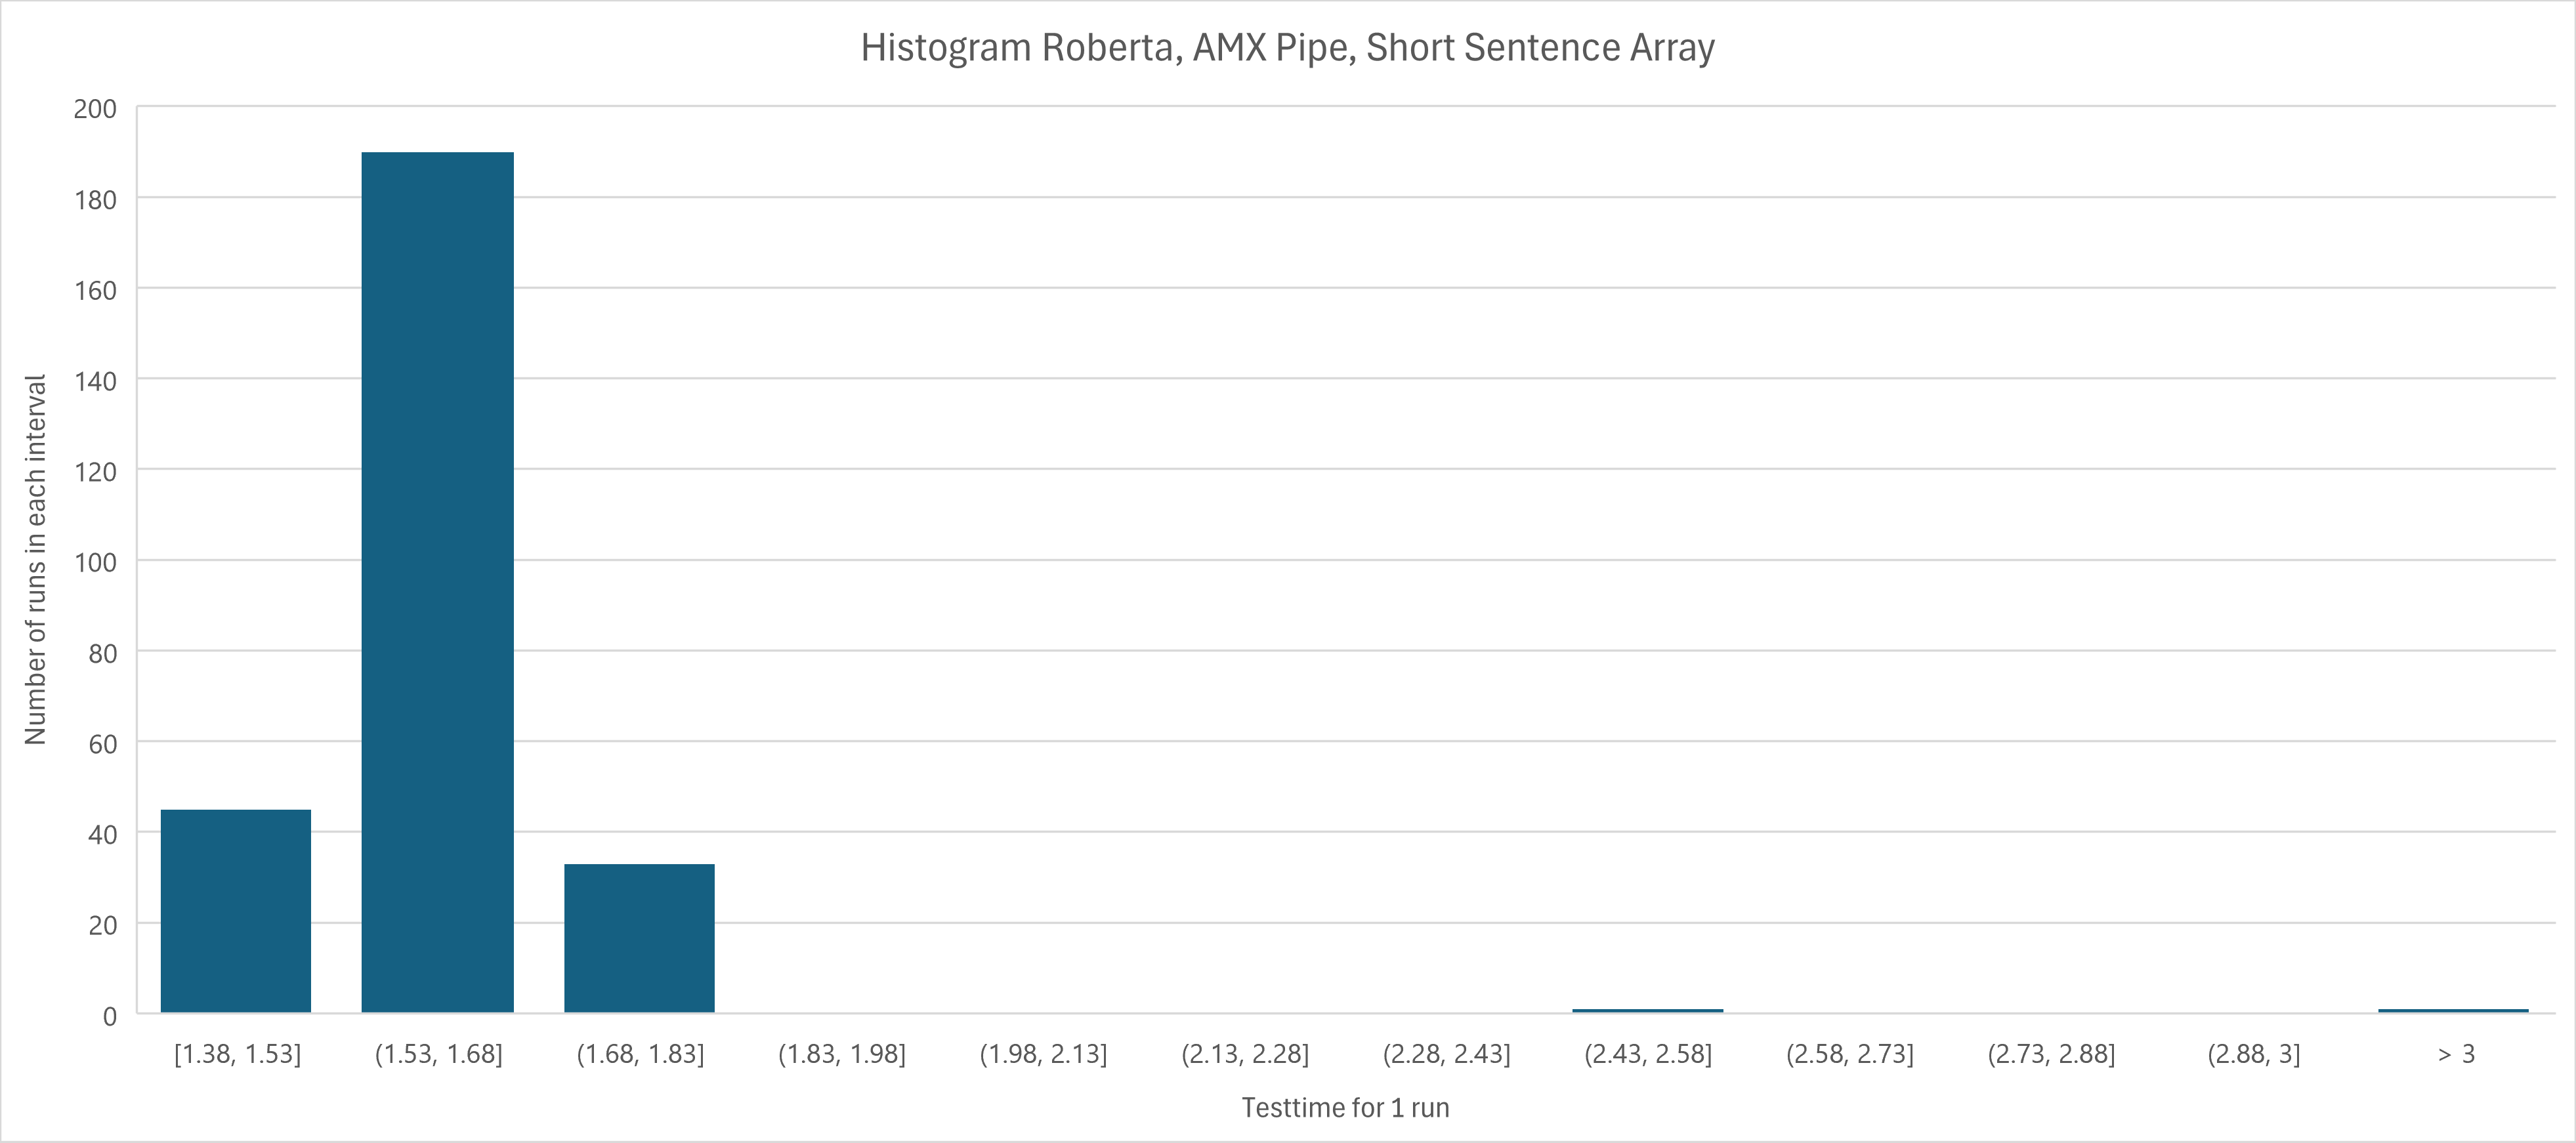
\includegraphics[width=\textwidth]{figures/Histogramm.png}
\caption{Shows the histogram of the short sentence array roBERTa AMX benchmark. The longest run to the right was over 6.4 seconds, but this would have made the diagram too big}
\label{fig:histogramm}
\end{figure}
A total of 2 out of 270 values were outliers but because some were so far outside the range 1.37s to 2.03s, the std dev was extremely high. Notably the longest run took 6.42 seconds almost 4 times as long as the mean. This one result increases the standard deviation from about 0.11 seconds to about 0.32 seconds. On the other hand the MAD only increases from about 0.03 to 0.04 seconds. The histogram clearly shows a clustering around about  1.65 seconds, which would not be appropriately represented by a standard deviation of 0.32 around the mean of 1.73 seconds. If two results are compared, they are checked for significant difference using Student’s two-sample, two-tailed t-test, the standard used with Pyperf, with an alpha equal to 0.05, the most commonly used threshold. 

\subsection{Benchmark Results}
The initial testing was done using Ubuntu 22.04 on both the guest system as well as the host system. The system later on had stability issues, which is why testing was then moved to a different platform as well as using Ubuntu 23.10 on both host and guest. This section will first describe the results from testing on Ubuntu 22.04 and then later on describe the results from Ubuntu 23.10. Comparisons will be made between TD and non-TD VMs using a common instruction set, as well as Intels AMX. The full benchmark results can be found at the KIT, which has the archives, or in the Github repository, which is currently located at

\myparagraph{Ubuntu 22.04}

The Benchmark results using distilBERT-base-uncased show a small performance loss of 2\% from a TD VM to a Non-TD VM. The performance difference fluctuates between the non-TD VM being 3\% slower on the long sentence array transformer pipe to being 5\% faster on the long sentence AMX pipe. Half the benchmarks did not have a t-value that make them significant. These were run 90 instead of 30 times as previously discussed as the first run had unexpected results. The first run had the TD VM about 18\% faster on average, after running them twice more the gap closed overall but only one suite had the expected outcome of the Non-TD VM running faster. These results could not be replicated on a different platform. The AMX variant was on average 29\% faster with the differences ranging from 19\% to 50\% faster.

The benchmark results using RoBERTa show a small performance loss of on average 1\% from a non-TD VM to a TD VM. The performance differs from about 5\% faster to 5\% slower. The absolute t-values range from 3.79 to 11.28. With 30 runs per test this results in p-values far below 0.01. All results except two were faster on non-TD VMs. The AMX accelerated pipe was faster on the TD VM on the short sentence array and long sentences. So while theses tests are statistically significant the difference in speed is not significant for real-world applications. AMX vs Non-AMX showed a speed increase of about 30\% in this benchmark, this is in line with the expected 1/3 speed increase.
\cref{fig:robertaUbuntu22.04} shows these miniscule differences quite well.
\begin{figure}
   \centering
       \includegraphics[width=.95\textwidth]{figures/Ubuntu22Roberta.png} 
 \caption{roberta-base inference times on Ubuntu 22.04}
 \label{fig:robertaUbuntu22.04}
\end{figure}


Both of the previous tests were done using an additional layer using a QEMU VM. Running the same benchmarks on the Host system directly averages an improvement of about 10\%. 
Due to the small margin between non-TD VMs and TD VM it was decided to test what disabling all TDX-related BIOS settings would have as an impact. This showed a significant speedup of on average 24\% using distillbert and 44\% using Roberta. The highest speed-up with 78\% was observed on the short-sentence array using Roberta. The difference was measurably slower using the AMX pipe with the distilbert TDX-enabled AMX pipe on the long-sentence being 5\% faster even. This difference was still inside the MAD, so could reasonably be explained with variations in testing. On average the non-AMX benchmarks were 53\% faster using distillbert and 71\% faster using Roberta. Figure \ref{fig:distillbertMADNONAMX} clearly shows the speed difference after disabling TDX in the BIOS. 
\begin{figure}
   \centering
       \includegraphics[width=.95\textwidth]{figures/distillbertMAD.png} 
 \caption{Distillbert Inference times on Ubuntu 22.04 without AMX}
 \label{fig:distillbertMADNONAMX}
\end{figure}
On the other hand Figure \ref{fig:distillbertMADAMX} shows no measurable speed difference after disabling TDX using the AMX-enabled Benchmarks. 
\begin{figure}
   \centering
       \includegraphics[width=.95\textwidth]{figures/distillbertMADAMX.png} 
 \caption{Distillbert Inference times on Ubuntu 22.04 using AMX}
 \label{fig:distillbertMADAMX}
\end{figure}
The AMX benchmarks were, using the geometric mean, similar in speed using distillbert, with a difference that was not statistically significant. The AMX benchmarks using Roberta were about 21\% faster. The overall speed-up was measurably faster than the initial observed AMX speedup, which indicates that this is not due to the omission of AMX in general but something different but having no speed-up using AMX with distillbert was an interesting result, which had no explainable reason. 

\myparagraph{Ubuntu 23.10}

All prior tests were done using Ubuntu 22.04 but due to the aforementioned stability issues a new platform with Ubuntu 23.10 was supplied by Intel. Rerunning the same tests using Ubuntu 23 the observed speed-up from a TD to TDX disabled diminished to just about 3\% with just TDX disabled and then an additional 3\% with memory-encryption disabled as well. These differences were small but the MAD on the measurements was even smaller, as can be seen in  \cref{fig:distillbertAMXUbuntu23}, so while these tests did not show large differences they appeared to be a lot more stable. 
\begin{figure}
   \centering
       \includegraphics[width=.95\textwidth]{figures/inferencedistillbertMADUbuntu23AMX.png} 
 \caption{Distillbert Inference times on Ubuntu 23 and Sapphire Rapid CPUs.Note: the apparent decrease in MAD is due to the logarithmic scale}
 \label{fig:distillbertAMXUbuntu23}
\end{figure}

A further examination was conducted on discernible execution time differences using a profiler on Ubuntu 23, but with just an eight percent speed difference, there was not much to observe. Minus the speed overhead of the profiler which was measured to be about 10 seconds, no matter the settings on the plattform, the execution took between 77 and 85 seconds, with the highest being TDX and memory encryption bypass enabled, which supposedly speeds up calculations. Some internal methods showed significant differences. The Intel Extension For Pytorch (IPEX) optimizer copy method saw timing increases of up to 400\%, this seems to be entirely due to activating TDX, as without TDX the timings were all within one percent of each other, enabling TDX without memory bypass increased this time by about 100\% and enabling bypass increases this a further 250\%. This method is called when AMX is enabled for the instruction set optimization. Total times for this IPEX optimization instruction can be seen in \ref{tab:IpexOpti}. The IPEX replacement method for linear transformation which takes most of the calculations shows small speed differences of about 5\% - which is about the same difference that was observed with the normal linear transformation method. The other methods all took about 5\% longer as well, which appears to be in line with the differences in memory access speed.
Having a look at the profiler results on the Azure cloud there are no clear results on overall speed but noticeably the IPEX copy and optimize instructions were once again measurably slower on the TD compared to a non-TD VM the optimization took about 20\% longer on the TD. This slow down is almost completely due to the time PyTorches clone function takes, which saw increases of around 1000\% in total and per call time. Memory encryption itself had close to no impact on the speed here. Neither did the Memory Encryption Bypass. Looking into the implementation of this function this is not expected. Clone creates shallow copies of a tensor, with the lower hierarchy memory being shared between the copies. With both the original and the copy being situated inside the TD, this is not a particularly demanding instruction. Its overhead should be similar in magnitude to the memory latency difference shown in \cref{tab:MemoryAccessSpeed}. Such a big overhead can be explained if a lot of context switching between encrypted and unencrypted memory has to be done, but this is not the case here.
\begin{table}
\centering
\resizebox{\textwidth}{!}{%
\begin{tabular}{ m{0.2\textwidth} m{0.2\textwidth} m{0.2\textwidth} m{0.2\textwidth} m{0.2\textwidth} m{0.2\textwidth}}
\toprule
& TD with ME Bypass & TD without ME Bypass & No-TD with ME & No-TD with ME Bypass & No Memory Encryption \\
\midrule
IPEX optimize total time & 1.21s & 0.597s & 0.28s & 0.278s & 0.284s \\
\midrule
PyTorch clone method & 1.01s & 0.397s & 0.079s & 0.077s & 0.077s \\
\bottomrule
\end{tabular}
}
\caption{Comparison of different timings of IPEX optimization method}
\label{tab:IpexOpti}
\end{table}


\subsection{Benchmarking TDX parts}

As stated in the previous section there were significant speed differences between having TDX enabled and disabled in the Bios but basically none when TDX was enabled in the Bios but disabled in the VM. Further investigations into what causes these speed-ups were necessary. As stated in \ref{sec:tdxBuildingBlocks} there were essentially two functionalities that could theoretically be tested independently from TDX, which could have a performance impact:
\begin{itemize}
    \item Total Memory Encryption 
    \item Intel VT, virtualization features
\end{itemize}
Intel \Gls{SGX} is only used for attestation purposes and thus does not have a performance impact. From TME and VT only TME was successfully tested as disabling VT prevented the system from booting.
For Total Memory Encryption, TDX and \Gls{SGX} were disabled, while Intel VT remained turned on. Stream \cite{mccalpin_memory_1995} and "PerformanceTest" \url{https://www.passmark.com/products/pt_linux/index.php} were used for benchmarking. Stream is the de facto standard for memory speed testing and PerformanceTest is a commonly used proprietary tool used to compare memory access speed. Using PerformanceTest there were small but measurable differences in speed of about 2.5\% for reading speed. The Writing speed remained within 1\% of each other. \cref{tab:MemoryAccessSpeed} shows the differences in more detail. The latency increased nearly 4.5\%.
\begin{table}
\centering
\resizebox{\textwidth}{!}{%
\begin{tabular}{ m{0.37\textwidth} m{0.25\textwidth} m{0.25\textwidth} m{0.13\textwidth}}
\toprule
Memory Benchmark Type & Memory encryption activated & Memory encryption deactivated & Difference \\
\midrule
Memory Allocation MB/s & 32445.11 & 33258.94 & 2.5\% \\
\midrule
Memory Read Cached MB/s & 27683.36 & 28148.14 & 1.6\% \\
\midrule
Memory Read Uncached MB/s & 10879.98 & 11123.77 & 2.2\% \\
\midrule
Memory Write Medium MB/s & 9592.82 & 9549.92 & -0.4\% \\
\midrule
Memory Write Threaded MB/s & 400550.9 & 411297.5 & 2.6\% \\
\midrule
Memory Latency ns & 64.3 & 61.4 & -4.5\% \\
\bottomrule
\end{tabular}
}
\caption{Results of Performancetests memory benchmark}
\label{tab:MemoryAccessSpeed}
\end{table}

With Stream, everything was tested disabled, just Memory Encryption enabled, and TDX completely enabled, and all three were within two percent of one another, with the encrypted memory being slightly faster than the other two. These results are most likely due to background noise of the system.

\begin{table}[]
    \centering
    \resizebox{\textwidth}{!}{%
    \begin{tabular}{m{0.2\textwidth} m{0.2\textwidth} m{0.2\textwidth} m{0.2\textwidth} m{0.2\textwidth} m{0.2\textwidth}}
    \hline
        Function & Best Rate MB/s Encrypted & Best Rate MB/s TDX enabled & Best Rate MB/s unencrypted & Best Rate Legacy VM MB/s & Best Rate TD MB/s \\ \hline
        Copy: & 292927.7 & 296714.7 & 299686.3 & 228281.2 & 209348.5979 \\ \hline
        Scale: & 291833.5 & 296603.3 & 298131.2 & 225828 & 206950.9938 \\ \hline
        Add: & 324643.9 & 318742.3 & 331304.6 & 250686.5 & 221401.8875 \\ \hline
        Triad: & 315635.1 & 329435.5 & 334132 & 232469.4 & 225711.5192 \\ \hline
        Normalized Geometric Mean & 1.418 & 1.437 & 1.462 & 1.085 & 1.000 \\ \hline
    \end{tabular}
    }
    \caption{Comparison of Memory Access speed using STREAM for various Non-VM settings as well as legacy VMs and TD}
\end{table}



\subsection{Security Attestation}

Attestation was not implemented or usable on the Intel Developer Cloud. Verifying usage of TDX was thus relying on the Linux Kernel itself as well as BIOS settings made by the user via an SSH connection. Without attestation the security benefits were theoretically not given. This was accepted as having bare-metal access meant being able to verify TDX activation directly and this hardware was only used for benchmarking.


\subsection{Performance Summary}
\label{Perf_EVal}

The initial testing on Ubuntu 22.04 showed the surprising result of having basically no slowdown or even a speedup when using TDX compared to a normal VM, while having TDX enabled in the BIOS. This results changed drastically when disabling TDX in the BIOS to about 30\% faster execution compared to the TD. These results persisted upon rerunning the tests on the same platform, although having the TD be faster on a different platform was not replicable. These results did not persist upon switching the platform, where the results were more inline with the expected five to ten percent difference, when using memory encryption. TD and non-TD VM, with the TDX being enabled stayed close to each other, which shows that there are basically no software-related slowdowns. A single method, which was necessary for the Intel AMX improved instructions, which only creates shallow copies showed significant slowdown of up to 1000\%. These were reproducible but it is unclear how they came to be. Overall the usage of a TD reduces inference speed by about ten percent, with most of this being due to the decreased memory speed, coming from the memory encryption. Using a non-TD on TDX enabled hardware offers no performance benefits. Additionally hosting a VM using QEMU decreases inference speed by about 30\% on its own, meaning the difference between TDX enabled and TDX disabled is a lot smaller than the difference between executing directly on the host vs inside a QEMU VM.




%% LaTeX2e class for student theses
%% sections/evaluation.tex
%% 
%% Karlsruhe Institute of Technology
%% Institute for Program Structures and Data Organization
%% Chair for Software Design and Quality (SDQ)
%%
%% Dr.-Ing. Erik Burger
%% burger@kit.edu
%%
%% Version 1.4, 2023-06-19

\chapter{Evaluation}
\label{ch:Evaluation}
This chapter will give a comparison of the three main implementations of self-hosted, a normal cloud implementation and a cloud implementation utilizing TDX.





%% LaTeX2e class for student theses
%% sections/conclusion.tex
%% 
%% Karlsruhe Institute of Technology
%% Institute for Program Structures and Data Organization
%% Chair for Software Design and Quality (SDQ)
%%
%% Dr.-Ing. Erik Burger
%% burger@kit.edu
%%
%% Version 1.4, 2023-06-19

\chapter{Conclusion}
\label{ch:Conclusion}

The general performance impacts of TDX are so small that they can be mostly ignored in day-to-day applications. Most users will not notice any differences, especially if memory encryption is used anyway. Comparing hosting on your own hardware, hosting in the cloud with TDX and hosting in the cloud without TDX, only about 10\% calculation time differences are to be expected. Bigger improvements could be made if a platform that does not need an additional VM layer can be made available, this could improve calculation times up to 30\%. There are however certain scenarios that could lead to a much higher overhead. As shown in \cref{performance} some instructions or methods can experience significant slowdowns when using TDX. It is unclear what leads to these slowdowns so the developer needs to check for themselves if they experience some unexplainable slow execution speeds.

These small performance decreases can potentially buy some great security guarantees, especially against software based attacks from a malicious Host or similar. TDX attestation, if implemented properly, seems to be found in its security assumptions. The threat model considers anyone with hardware access as untrusted, this includes the cloud provider. As discussed previously TDX can not protect against all hardware attacks, meaning that anyone with hardware access can extract information from a TD if they know how to implement certain kinds of attacks, discussed in \cref{Security Analysis}. Similarly someone with hardware access can also extract information on self-hosted applications. The assumption that the cloud provider can be completely removed from the list of trusted parties, as claimed by Intel, is thus at best an exaggeration and at worst just false. Looking further into one implementation of Intel TDX these issues become even more pronounced, a lot of trust has to be put into Microsoft proprietary code regarding the attestation. It was not possible for me to create a quote that was completely independent of any Microsoft code. As it stands currently it is not recommended to rely upon TDX, to remove the cloud provider from the list of trusted parties.


\myparagraph{Outlook}

This thesis focused on simple TDX implementations. With TDX having just been released, most of those implementations are still in their infancy and problems are to be expected. Hopefully in the future some of those, that have been highlighted in this thesis and those that have not been will be fixed. Nonetheless there are still additional things that can be looked at. The implementation of TDX in Ubuntu 22 appears to cause instability issues and also performance defiencies compared to the implementation in Ubuntu 23. Having a deeper look at the differences between those two could grant significant improvements. Additionally, comparisons between the different hardware Confidential Computing hardware providers are necessary to being able to make the decision for or against Confidential Computing. Additionally looking into the implementation of PyTorch to figure out why its copy function experiences such significant slowdown is advised. 

For the future Intel has planned a cooperation with Nvidia to bring Confidential Computing and AI closer together \url{https://community.intel.com/t5/Blogs/Products-and-Solutions/Security/Intel-Nvidia-Collaborate-to-Deliver-Confidential-AI-Solutions/post/1500066}. With the release of Intel attestation for Nvidia hardware to be planned in the first half of 2024, confidential computing on GPU hardware could be a possibility. Intel and Nvidia have yet to release architecture specifications for their collaboration but their security promises and assumptions will have to be tested then. If implementation could be simplified for the average user this could be a great step into the right direction for data security. The dangers of dedicated GPUs and the possible performance losses with establishing a secure communication between CPU and GPU are a challenge that will have to be solved first. Silberstein et al. highlighted the dangers of insecure communication and other problems with dedicated GPUs in their 2020 paper \cite{zhu_enabling_2020}.

Additionally this thesis was limited in regard to the amount of performancetesting that was feasible. More I/O heavy workloads and even some GPU-bound workloads could be tested. Implementing ways to calculate on a non-trusted GPU, while maintaining data confidentiality is still an ongoing line of research, which could be even more interesting in the future, but it still has security and performance problems, compare \cite{ogburn_homomorphic_2013} and \cite{li_security_2020} for more information on this.







%% --------------------
%% |   Bibliography   |
%% --------------------

%% Add entry to the table of contents for the bibliography
\printbibliography[heading=bibintoc]

%% ----------------
%% |   Appendix   |
%% ----------------
\appendix
%% LaTeX2e class for student theses
%% sections/apendix.tex
%% 
%% Karlsruhe Institute of Technology
%% Institute for Program Structures and Data Organization
%% Chair for Software Design and Quality (SDQ)
%%
%% Dr.-Ing. Erik Burger
%% burger@kit.edu
%%
%% Version 1.4, 2023-06-19

\iflanguage{english}
{\chapter{Appendix}}    % english style
{\chapter{Anhang}}      % german style
\label{chap:appendix}


%% -------------------
%% | Example content |
%% -------------------

\section{Security}

\paragraph{Microsoft Azure Attestation JWT verification}
\label{jwt}
\begin{lstlisting}[language=json]
    {
  "attester_tcb_status": "UpToDate",
  "dbgstat": "disabled",
  "eat_profile": "https://aka.ms/maa-eat-profile-tdxvm",
  "exp": 1705689946,
  "iat": 1705661146,
  "intuse": "generic",
  "iss": "https://sharedeus2e.eus2e.attest.azure.net",
  "jti": "01bd3ce9833084751244fbde515a9c410f2af383ee483734b410d8c031120018",
  "nbf": 1705661146,
  "tdx_mrconfigid": "000000000000000000000000000000000000000000000000000000000000000000000000000000000000000000000000",
  "tdx_mrowner": "000000000000000000000000000000000000000000000000000000000000000000000000000000000000000000000000",
  "tdx_mrownerconfig": "000000000000000000000000000000000000000000000000000000000000000000000000000000000000000000000000",
  "tdx_mrseam": "360304d34a16aace0a18e09ad2d07d2b9fd3c174378e5bf108388079827f89ff62acc5f8c473dd40706324834e202946",
  "tdx_mrsignerseam": "000000000000000000000000000000000000000000000000000000000000000000000000000000000000000000000000",
  "tdx_mrtd": "024a32b070383331181619fa387cb4d55d1e38879f989933055ccad5bc2db795d1737b66205949d15469dc8c1ba7ab7b",
  "tdx_report_data": "c90f98ba8ab80c7b442b6b8eb30af54e0508077b11adb525af6dfbcc8714e52a0000000000000000000000000000000000000000000000000000000000000000",
  "tdx_rtmr0": "000000000000000000000000000000000000000000000000000000000000000000000000000000000000000000000000",
  "tdx_rtmr1": "000000000000000000000000000000000000000000000000000000000000000000000000000000000000000000000000",
  "tdx_rtmr2": "000000000000000000000000000000000000000000000000000000000000000000000000000000000000000000000000",
  "tdx_rtmr3": "000000000000000000000000000000000000000000000000000000000000000000000000000000000000000000000000",
  "tdx_seam_attributes": "0000000000000000",
  "tdx_seamsvn": 258,
  "tdx_td_attributes": "0000000000000000",
  "tdx_td_attributes_debug": false,
  "tdx_td_attributes_key_locker": false,
  "tdx_td_attributes_perfmon": false,
  "tdx_td_attributes_protection_keys": false,
  "tdx_td_attributes_septve_disable": false,
  "tdx_tee_tcb_svn": "02010600000000000000000000000000",
  "tdx_xfam": "e718060000000000",
  "x-ms-attestation-type": "tdxvm",
  "x-ms-compliance-status": "azure-compliant-cvm",
  "x-ms-policy-hash": "9NY0VnTQ-IiBriBplVUpFbczcDaEBUwsiFYAzHu_gco",
  "x-ms-runtime": {
    "keys": [
      {
        "e": "AQAB",
        "key_ops": [
          "sign"
        ],
        "kid": "HCLAkPub",
        "kty": "RSA",
        "n": "p4ig6gABSEmW9oijgg37ZDj7ZcaxnyN2h9KTHLAUYJnoP-42Hi209p1RdiL3HSWdRzzSDuXKjQw2kzlmcX1XfBq9-3-L-CVoyCvpiin-6k9L_Rbu0upEiBnIw2IzJ5N6EZx7zfX8vdh76MMnT-_U2Pd2psoiUufzNvs2-5d0QB5NyTuCnXbWD_yWb1OQWZAPioXEIyR13ic-FxPt5UiGG6kBjGp41rqlEQ0B_tsfn3e19_lTx76wVfEkEOw5Yq60rTyNuxiOnR59reaxXui0qJTOkoiDOJ-tHLffY_jTT-8EUFtWS1mcPoye2uKRhAI99xjTWg88Ft4sIUv8stOTvw"
      },
      {
        "e": "AQAB",
        "key_ops": [
          "encrypt"
        ],
        "kid": "HCLEkPub",
        "kty": "RSA",
        "n": "4galYAAA8uQxZCGg7qvvY0hcck4UY-EPiqWyxkHH0rMyQJh2nWuriu5wrh4JPPy6HvtX5M-mr5ecHPYf4S0qTOcqWZX01Uj8Ky1sbvA6g1GELe0Jdqf9piQDmS90dGwR6PItHMObnejzBocweHxkuSm7pGSuOAniX6KDid1hsxED5gYLxg2wHAXFICz9UZOTQ6FZmezVz0Krpr2AF4fKawOIaQSwNl7GIjH09x7rFRP2H1zOW6sJYAIAIT7F7vfncB3ZpPHUrU9U-qSQC2LZBRtjuBaKG-kGU6jAOkMC8aXu_pb99vgrrJpn2Nf8VodePJ7gzwladZjCnflyUWViYw"
      }
    ],
    "user-data": "00000000000000000000000000000000000000000000000000000000000000000000000000000000000000000000000000000000000000000000000000000000",
    "vm-configuration": {
      "console-enabled": true,
      "root-cert-thumbprint": "6nZZnYaJc4KqUZ_yvA-mucFdYNouvlPnITnNMXsHl-0",
      "secure-boot": true,
      "tpm-enabled": true,
      "tpm-persisted": true,
      "vmUniqueId": "C540205B-C5A0-4380-A0F9-7ECA9B91113A"
    }
  },
  "x-ms-ver": "1.0"
}
\end{lstlisting}


\section{Benchmark Results}
\subsection{Ubuntu 22.10}
\subsubsection{Roberta Non TD}
\label{sec:appendix:benchmarks:roberta}

\begin{lstlisting}[language=json]
Number of benchmarks: 8
Total duration: 2 hour 57 min 25.7 sec
Start date: 2023-12-19 05:34:37
End date: 2023-12-19 14:36:43

Transformer pipe, short sentence, roberta-base
----------------------------------------------

Total duration: 3 min 45.4 sec
Start date: 2023-12-19 05:34:37
End date: 2023-12-19 06:22:10
Raw value minimum: 1.37 sec
Raw value maximum: 2.04 sec

Number of calibration run: 1
Number of run with values: 30
Total number of run: 31

Number of warmup per run: 1
Number of value per run: 3
Loop iterations per value: 5 (1 outer-loop x 5 inner-loops)
Total number of values: 90

Minimum:         274 ms
Median +- MAD:   365 ms +- 10 ms
Mean +- std dev: 361 ms +- 21 ms
Maximum:         407 ms

  0th percentile: 274 ms (-24% of the mean) -- minimum
  5th percentile: 323 ms (-11% of the mean)
 25th percentile: 354 ms (-2% of the mean) -- Q1
 50th percentile: 365 ms (+1% of the mean) -- median
 75th percentile: 375 ms (+4% of the mean) -- Q3
 95th percentile: 383 ms (+6% of the mean)
100th percentile: 407 ms (+13% of the mean) -- maximum

Number of outlier (out of 322 ms..407 ms): 6

Transformer pipe, long sentence, roberta-base
---------------------------------------------

Total duration: 6 min 42.5 sec
Start date: 2023-12-19 06:23:52
End date: 2023-12-19 07:14:45
Raw value minimum: 2.86 sec
Raw value maximum: 3.73 sec

Number of calibration run: 1
Number of run with values: 30
Total number of run: 31

Number of warmup per run: 1
Number of value per run: 3
Loop iterations per value: 5 (1 outer-loop x 5 inner-loops)
Total number of values: 90

Minimum:         571 ms
Median +- MAD:   669 ms +- 31 ms
Mean +- std dev: 661 ms +- 44 ms
Maximum:         746 ms

  0th percentile: 571 ms (-14% of the mean) -- minimum
  5th percentile: 593 ms (-10% of the mean)
 25th percentile: 617 ms (-7% of the mean) -- Q1
 50th percentile: 669 ms (+1% of the mean) -- median
 75th percentile: 695 ms (+5% of the mean) -- Q3
 95th percentile: 724 ms (+9% of the mean)
100th percentile: 746 ms (+13% of the mean) -- maximum

Number of outlier (out of 500 ms..811 ms): 0

Transformer pipe, short sentence array, roberta-base
----------------------------------------------------

Total duration: 30 min 17.6 sec
Start date: 2023-12-19 07:17:33
End date: 2023-12-19 08:32:20
Raw value minimum: 12.8 sec
Raw value maximum: 16.2 sec

Number of calibration run: 1
Number of run with values: 30
Total number of run: 31

Number of warmup per run: 1
Number of value per run: 3
Loop iterations per value: 5 (1 outer-loop x 5 inner-loops)
Total number of values: 90

Minimum:         2.55 sec
Median +- MAD:   2.95 sec +- 0.10 sec
Mean +- std dev: 2.94 sec +- 0.16 sec
Maximum:         3.25 sec

  0th percentile: 2.55 sec (-13% of the mean) -- minimum
  5th percentile: 2.67 sec (-9% of the mean)
 25th percentile: 2.84 sec (-3% of the mean) -- Q1
 50th percentile: 2.95 sec (+0% of the mean) -- median
 75th percentile: 3.05 sec (+4% of the mean) -- Q3
 95th percentile: 3.21 sec (+9% of the mean)
100th percentile: 3.25 sec (+10% of the mean) -- maximum

Number of outlier (out of 2.54 sec..3.36 sec): 0

Transformer pipe, long sentence array, roberta-base
---------------------------------------------------

Total duration: 56 min 21.3 sec
Start date: 2023-12-19 08:35:33
End date: 2023-12-19 10:15:29
Raw value minimum: 24.7 sec
Raw value maximum: 30.5 sec

Number of calibration run: 1
Number of run with values: 30
Total number of run: 31

Number of warmup per run: 1
Number of value per run: 3
Loop iterations per value: 5 (1 outer-loop x 5 inner-loops)
Total number of values: 90

Minimum:         4.94 sec
Median +- MAD:   5.49 sec +- 0.16 sec
Mean +- std dev: 5.48 sec +- 0.23 sec
Maximum:         6.09 sec

  0th percentile: 4.94 sec (-10% of the mean) -- minimum
  5th percentile: 5.16 sec (-6% of the mean)
 25th percentile: 5.32 sec (-3% of the mean) -- Q1
 50th percentile: 5.49 sec (+0% of the mean) -- median
 75th percentile: 5.64 sec (+3% of the mean) -- Q3
 95th percentile: 5.83 sec (+6% of the mean)
100th percentile: 6.09 sec (+11% of the mean) -- maximum

Number of outlier (out of 4.83 sec..6.13 sec): 0

AMX pipe, short sentence, roberta-base
--------------------------------------

Total duration: 2 min 35.2 sec
Start date: 2023-12-19 10:15:15
End date: 2023-12-19 11:01:19
Raw value minimum: 1.15 sec
Raw value maximum: 1.39 sec

Number of calibration run: 1
Number of run with values: 30
Total number of run: 31

Number of warmup per run: 1
Number of value per run: 3
Loop iterations per value: 5 (1 outer-loop x 5 inner-loops)
Total number of values: 90

Minimum:         231 ms
Median +- MAD:   248 ms +- 10 ms
Mean +- std dev: 249 ms +- 13 ms
Maximum:         278 ms

  0th percentile: 231 ms (-7% of the mean) -- minimum
  5th percentile: 232 ms (-7% of the mean)
 25th percentile: 238 ms (-4% of the mean) -- Q1
 50th percentile: 248 ms (-0% of the mean) -- median
 75th percentile: 257 ms (+3% of the mean) -- Q3
 95th percentile: 274 ms (+10% of the mean)
100th percentile: 278 ms (+12% of the mean) -- maximum

Number of outlier (out of 209 ms..286 ms): 0

AMX pipe, long sentence, roberta-base
-------------------------------------

Total duration: 6 min 25.9 sec
Start date: 2023-12-19 11:03:00
End date: 2023-12-19 11:53:03
Raw value minimum: 2.92 sec
Raw value maximum: 3.40 sec

Number of calibration run: 1
Number of run with values: 30
Total number of run: 31

Number of warmup per run: 1
Number of value per run: 3
Loop iterations per value: 5 (1 outer-loop x 5 inner-loops)
Total number of values: 90

Minimum:         583 ms
Median +- MAD:   622 ms +- 9 ms
Mean +- std dev: 623 ms +- 19 ms
Maximum:         680 ms

  0th percentile: 583 ms (-6% of the mean) -- minimum
  5th percentile: 594 ms (-5% of the mean)
 25th percentile: 613 ms (-2% of the mean) -- Q1
 50th percentile: 622 ms (-0% of the mean) -- median
 75th percentile: 632 ms (+1% of the mean) -- Q3
 95th percentile: 654 ms (+5% of the mean)
100th percentile: 680 ms (+9% of the mean) -- maximum

Number of outlier (out of 585 ms..660 ms): 7

AMX pipe, short sentence array, roberta-base
--------------------------------------------

Total duration: 20 min 38.7 sec
Start date: 2023-12-19 11:55:23
End date: 2023-12-19 12:58:20
Raw value minimum: 9.28 sec
Raw value maximum: 10.8 sec

Number of calibration run: 1
Number of run with values: 30
Total number of run: 31

Number of warmup per run: 1
Number of value per run: 3
Loop iterations per value: 5 (1 outer-loop x 5 inner-loops)
Total number of values: 90

Minimum:         1.86 sec
Median +- MAD:   1.98 sec +- 0.04 sec
Mean +- std dev: 1.98 sec +- 0.07 sec
Maximum:         2.16 sec

  0th percentile: 1.86 sec (-6% of the mean) -- minimum
  5th percentile: 1.88 sec (-5% of the mean)
 25th percentile: 1.94 sec (-2% of the mean) -- Q1
 50th percentile: 1.98 sec (-0% of the mean) -- median
 75th percentile: 2.03 sec (+2% of the mean) -- Q3
 95th percentile: 2.10 sec (+6% of the mean)
100th percentile: 2.16 sec (+9% of the mean) -- maximum

Number of outlier (out of 1.80 sec..2.16 sec): 0

AMX pipe, long sentence array, roberta-base
-------------------------------------------

Total duration: 50 min 39.0 sec
Start date: 2023-12-19 13:01:24
End date: 2023-12-19 14:36:43
Raw value minimum: 21.8 sec
Raw value maximum: 26.4 sec

Number of calibration run: 1
Number of run with values: 30
Total number of run: 31

Number of warmup per run: 1
Number of value per run: 3
Loop iterations per value: 5 (1 outer-loop x 5 inner-loops)
Total number of values: 90

Minimum:         4.37 sec
Median +- MAD:   4.92 sec +- 0.10 sec
Mean +- std dev: 4.89 sec +- 0.16 sec
Maximum:         5.27 sec

  0th percentile: 4.37 sec (-11% of the mean) -- minimum
  5th percentile: 4.63 sec (-5% of the mean)
 25th percentile: 4.80 sec (-2% of the mean) -- Q1
 50th percentile: 4.92 sec (+0% of the mean) -- median
 75th percentile: 5.00 sec (+2% of the mean) -- Q3
 95th percentile: 5.11 sec (+4% of the mean)
100th percentile: 5.27 sec (+8% of the mean) -- maximum
\end{lstlisting}

\subsubsection{Roberta TD}
\begin{lstlisting}[language=json]
Number of benchmarks: 8
Total duration: 2 hour 59 min 0.6 sec
Start date: 2023-12-19 05:32:58
End date: 2023-12-19 14:37:09

Transformer pipe, short sentence, roberta-base
----------------------------------------------

Total duration: 3 min 53.6 sec
Start date: 2023-12-19 05:32:58
End date: 2023-12-19 06:20:59
Raw value minimum: 1.44 sec
Raw value maximum: 2.23 sec

Number of calibration run: 1
Number of run with values: 30
Total number of run: 31

Number of warmup per run: 1
Number of value per run: 3
Loop iterations per value: 5 (1 outer-loop x 5 inner-loops)
Total number of values: 90

Minimum:         288 ms
Median +- MAD:   383 ms +- 15 ms
Mean +- std dev: 378 ms +- 26 ms
Maximum:         446 ms

  0th percentile: 288 ms (-24% of the mean) -- minimum
  5th percentile: 343 ms (-9% of the mean)
 25th percentile: 365 ms (-3% of the mean) -- Q1
 50th percentile: 383 ms (+1% of the mean) -- median
 75th percentile: 393 ms (+4% of the mean) -- Q3
 95th percentile: 412 ms (+9% of the mean)
100th percentile: 446 ms (+18% of the mean) -- maximum

Number of outlier (out of 321 ms..437 ms): 4

Transformer pipe, long sentence, roberta-base
---------------------------------------------

Total duration: 7 min 8.4 sec
Start date: 2023-12-19 06:22:43
End date: 2023-12-19 07:13:48
Raw value minimum: 3.20 sec
Raw value maximum: 3.78 sec

Number of calibration run: 1
Number of run with values: 30
Total number of run: 31

Number of warmup per run: 1
Number of value per run: 3
Loop iterations per value: 5 (1 outer-loop x 5 inner-loops)
Total number of values: 90

Minimum:         640 ms
Median +- MAD:   692 ms +- 16 ms
Mean +- std dev: 690 ms +- 25 ms
Maximum:         756 ms

  0th percentile: 640 ms (-7% of the mean) -- minimum
  5th percentile: 645 ms (-7% of the mean)
 25th percentile: 673 ms (-2% of the mean) -- Q1
 50th percentile: 692 ms (+0% of the mean) -- median
 75th percentile: 706 ms (+2% of the mean) -- Q3
 95th percentile: 727 ms (+5% of the mean)
100th percentile: 756 ms (+10% of the mean) -- maximum

Number of outlier (out of 623 ms..756 ms): 0

Transformer pipe, short sentence array, roberta-base
----------------------------------------------------

Total duration: 31 min 27.1 sec
Start date: 2023-12-19 07:16:26
End date: 2023-12-19 08:32:55
Raw value minimum: 13.4 sec
Raw value maximum: 16.8 sec

Number of calibration run: 1
Number of run with values: 30
Total number of run: 31

Number of warmup per run: 1
Number of value per run: 3
Loop iterations per value: 5 (1 outer-loop x 5 inner-loops)
Total number of values: 90

Minimum:         2.68 sec
Median +- MAD:   3.05 sec +- 0.10 sec
Mean +- std dev: 3.05 sec +- 0.15 sec
Maximum:         3.37 sec

  0th percentile: 2.68 sec (-12% of the mean) -- minimum
  5th percentile: 2.81 sec (-8% of the mean)
 25th percentile: 2.97 sec (-3% of the mean) -- Q1
 50th percentile: 3.05 sec (-0% of the mean) -- median
 75th percentile: 3.16 sec (+3% of the mean) -- Q3
 95th percentile: 3.27 sec (+7% of the mean)
100th percentile: 3.37 sec (+10% of the mean) -- maximum

Number of outlier (out of 2.70 sec..3.44 sec): 1

Transformer pipe, long sentence array, roberta-base
---------------------------------------------------

Total duration: 57 min 47.0 sec
Start date: 2023-12-19 08:36:09
End date: 2023-12-19 10:18:22
Raw value minimum: 25.5 sec
Raw value maximum: 31.6 sec

Number of calibration run: 1
Number of run with values: 30
Total number of run: 31

Number of warmup per run: 1
Number of value per run: 3
Loop iterations per value: 5 (1 outer-loop x 5 inner-loops)
Total number of values: 90

Minimum:         5.11 sec
Median +- MAD:   5.58 sec +- 0.22 sec
Mean +- std dev: 5.62 sec +- 0.28 sec
Maximum:         6.33 sec

  0th percentile: 5.11 sec (-9% of the mean) -- minimum
  5th percentile: 5.24 sec (-7% of the mean)
 25th percentile: 5.40 sec (-4% of the mean) -- Q1
 50th percentile: 5.58 sec (-1% of the mean) -- median
 75th percentile: 5.85 sec (+4% of the mean) -- Q3
 95th percentile: 6.05 sec (+8% of the mean)
100th percentile: 6.33 sec (+13% of the mean) -- maximum

Number of outlier (out of 4.73 sec..6.52 sec): 0

AMX pipe, short sentence, roberta-base
--------------------------------------

Total duration: 2 min 31.3 sec
Start date: 2023-12-19 10:18:10
End date: 2023-12-19 11:04:14
Raw value minimum: 1.12 sec
Raw value maximum: 1.44 sec

Number of calibration run: 1
Number of run with values: 30
Total number of run: 31

Number of warmup per run: 1
Number of value per run: 3
Loop iterations per value: 5 (1 outer-loop x 5 inner-loops)
Total number of values: 90

Minimum:         225 ms
Median +- MAD:   240 ms +- 4 ms
Mean +- std dev: 241 ms +- 11 ms
Maximum:         287 ms

  0th percentile: 225 ms (-7% of the mean) -- minimum
  5th percentile: 229 ms (-5% of the mean)
 25th percentile: 235 ms (-2% of the mean) -- Q1
 50th percentile: 240 ms (-1% of the mean) -- median
 75th percentile: 243 ms (+1% of the mean) -- Q3
 95th percentile: 271 ms (+13% of the mean)
100th percentile: 287 ms (+19% of the mean) -- maximum

Number of outlier (out of 224 ms..254 ms): 6

AMX pipe, long sentence, roberta-base
-------------------------------------

Total duration: 6 min 9.6 sec
Start date: 2023-12-19 11:05:54
End date: 2023-12-19 11:55:49
Raw value minimum: 2.81 sec
Raw value maximum: 3.22 sec

Number of calibration run: 1
Number of run with values: 30
Total number of run: 31

Number of warmup per run: 1
Number of value per run: 3
Loop iterations per value: 5 (1 outer-loop x 5 inner-loops)
Total number of values: 90

Minimum:         561 ms
Median +- MAD:   594 ms +- 8 ms
Mean +- std dev: 594 ms +- 15 ms
Maximum:         644 ms

  0th percentile: 561 ms (-6% of the mean) -- minimum
  5th percentile: 568 ms (-4% of the mean)
 25th percentile: 585 ms (-2% of the mean) -- Q1
 50th percentile: 594 ms (+0% of the mean) -- median
 75th percentile: 602 ms (+1% of the mean) -- Q3
 95th percentile: 621 ms (+4% of the mean)
100th percentile: 644 ms (+8% of the mean) -- maximum

Number of outlier (out of 560 ms..627 ms): 2

AMX pipe, short sentence array, roberta-base
--------------------------------------------

Total duration: 20 min 46.5 sec
Start date: 2023-12-19 11:58:01
End date: 2023-12-19 13:01:05
Raw value minimum: 9.09 sec
Raw value maximum: 11.3 sec

Number of calibration run: 1
Number of run with values: 30
Total number of run: 31

Number of warmup per run: 1
Number of value per run: 3
Loop iterations per value: 5 (1 outer-loop x 5 inner-loops)
Total number of values: 90

Minimum:         1.82 sec
Median +- MAD:   2.04 sec +- 0.04 sec
Mean +- std dev: 2.03 sec +- 0.08 sec
Maximum:         2.27 sec

  0th percentile: 1.82 sec (-10% of the mean) -- minimum
  5th percentile: 1.91 sec (-6% of the mean)
 25th percentile: 1.99 sec (-2% of the mean) -- Q1
 50th percentile: 2.04 sec (+0% of the mean) -- median
 75th percentile: 2.07 sec (+2% of the mean) -- Q3
 95th percentile: 2.16 sec (+7% of the mean)
100th percentile: 2.27 sec (+12% of the mean) -- maximum

Number of outlier (out of 1.87 sec..2.18 sec): 4

AMX pipe, long sentence array, roberta-base
-------------------------------------------

Total duration: 49 min 17.0 sec
Start date: 2023-12-19 13:04:16
End date: 2023-12-19 14:37:09
Raw value minimum: 17.2 sec
Raw value maximum: 25.5 sec

Number of calibration run: 1
Number of run with values: 30
Total number of run: 31

Number of warmup per run: 1
Number of value per run: 3
Loop iterations per value: 5 (1 outer-loop x 5 inner-loops)
Total number of values: 90

Minimum:         3.43 sec
Median +- MAD:   4.83 sec +- 0.10 sec
Mean +- std dev: 4.76 sec +- 0.29 sec
Maximum:         5.10 sec

  0th percentile: 3.43 sec (-28% of the mean) -- minimum
  5th percentile: 4.40 sec (-8% of the mean)
 25th percentile: 4.73 sec (-1% of the mean) -- Q1
 50th percentile: 4.83 sec (+1% of the mean) -- median
 75th percentile: 4.93 sec (+3% of the mean) -- Q3
 95th percentile: 5.04 sec (+6% of the mean)
100th percentile: 5.10 sec (+7% of the mean) -- maximum

Number of outlier (out of 4.42 sec..5.23 sec): 6
\end{lstlisting}

\subsection{Distillbert Non TD results}
\label{app:bert}
\begin{lstlisting}[language=json]
    Number of benchmarks: 8
Total duration: 4 hour 17 min 0.8 sec
Start date: 2023-12-18 10:45:48
End date: 2023-12-20 18:58:05

Transformer pipe, short sentence, distilbert-base-uncased
---------------------------------------------------------

Total duration: 4 min 45.1 sec
Start date: 2023-12-18 10:45:48
End date: 2023-12-20 14:57:20
Raw value minimum: 588 ms
Raw value maximum: 963 ms

Number of calibration run: 3
Number of run with values: 90
Total number of run: 93

Number of warmup per run: 1
Number of value per run: 3
Loop iterations per value: 5 (1 outer-loop x 5 inner-loops)
Total number of values: 270

Minimum:         118 ms
Median +- MAD:   150 ms +- 12 ms
Mean +- std dev: 152 ms +- 16 ms
Maximum:         193 ms

  0th percentile: 118 ms (-23% of the mean) -- minimum
  5th percentile: 130 ms (-15% of the mean)
 25th percentile: 140 ms (-8% of the mean) -- Q1
 50th percentile: 150 ms (-1% of the mean) -- median
 75th percentile: 164 ms (+8% of the mean) -- Q3
 95th percentile: 179 ms (+17% of the mean)
100th percentile: 193 ms (+27% of the mean) -- maximum

Number of outlier (out of 105 ms..199 ms): 0

WARNING: the benchmark result may be unstable
* the standard deviation (15.6 ms) is 10% of the mean (152 ms)

Try to rerun the benchmark with more runs, values and/or loops.
Run 'python3 -m pyperf system tune' command to reduce the system jitter.
Use pyperf stats, pyperf dump and pyperf hist to analyze results.
Use --quiet option to hide these warnings.

Transformer pipe, long sentence, distilbert-base-uncased
--------------------------------------------------------

Total duration: 10 min 22.7 sec
Start date: 2023-12-18 12:36:35
End date: 2023-12-20 15:23:53
Raw value minimum: 1.30 sec
Raw value maximum: 1.98 sec

Number of calibration run: 3
Number of run with values: 90
Total number of run: 93

Number of warmup per run: 1
Number of value per run: 3
Loop iterations per value: 5 (1 outer-loop x 5 inner-loops)
Total number of values: 270

Minimum:         259 ms
Median +- MAD:   337 ms +- 23 ms
Mean +- std dev: 332 ms +- 32 ms
Maximum:         397 ms

  0th percentile: 259 ms (-22% of the mean) -- minimum
  5th percentile: 278 ms (-16% of the mean)
 25th percentile: 307 ms (-8% of the mean) -- Q1
 50th percentile: 337 ms (+1% of the mean) -- median
 75th percentile: 357 ms (+8% of the mean) -- Q3
 95th percentile: 378 ms (+14% of the mean)
100th percentile: 397 ms (+19% of the mean) -- maximum

Number of outlier (out of 230 ms..434 ms): 0

Transformer pipe, short sentence array, distilbert-base-uncased
---------------------------------------------------------------

Total duration: 42 min 29.8 sec
Start date: 2023-12-18 14:34:31
End date: 2023-12-20 16:02:00
Raw value minimum: 5.32 sec
Raw value maximum: 9.58 sec

Number of calibration run: 3
Number of run with values: 90
Total number of run: 93

Number of warmup per run: 1
Number of value per run: 3
Loop iterations per value: 5 (1 outer-loop x 5 inner-loops)
Total number of values: 270

Minimum:         1.06 sec
Median +- MAD:   1.34 sec +- 0.09 sec
Mean +- std dev: 1.37 sec +- 0.17 sec
Maximum:         1.92 sec

  0th percentile: 1.06 sec (-23% of the mean) -- minimum
  5th percentile: 1.18 sec (-14% of the mean)
 25th percentile: 1.25 sec (-9% of the mean) -- Q1
 50th percentile: 1.34 sec (-3% of the mean) -- median
 75th percentile: 1.44 sec (+5% of the mean) -- Q3
 95th percentile: 1.73 sec (+26% of the mean)
100th percentile: 1.92 sec (+40% of the mean) -- maximum

Number of outlier (out of 969 ms..1723 ms): 15

WARNING: the benchmark result may be unstable
* the standard deviation (170 ms) is 12% of the mean (1.37 sec)

Try to rerun the benchmark with more runs, values and/or loops.
Run 'python3 -m pyperf system tune' command to reduce the system jitter.
Use pyperf stats, pyperf dump and pyperf hist to analyze results.
Use --quiet option to hide these warnings.

Transformer pipe, long sentence array, distilbert-base-uncased
--------------------------------------------------------------

Total duration: 1 hour 27 min 40.1 sec
Start date: 2023-12-18 16:45:44
End date: 2023-12-20 16:55:12
Raw value minimum: 11.8 sec
Raw value maximum: 16.3 sec

Number of calibration run: 3
Number of run with values: 90
Total number of run: 93

Number of warmup per run: 1
Number of value per run: 3
Loop iterations per value: 5 (1 outer-loop x 5 inner-loops)
Total number of values: 270

Minimum:         2.36 sec
Median +- MAD:   2.80 sec +- 0.12 sec
Mean +- std dev: 2.81 sec +- 0.17 sec
Maximum:         3.25 sec

  0th percentile: 2.36 sec (-16% of the mean) -- minimum
  5th percentile: 2.54 sec (-10% of the mean)
 25th percentile: 2.69 sec (-4% of the mean) -- Q1
 50th percentile: 2.80 sec (-0% of the mean) -- median
 75th percentile: 2.93 sec (+4% of the mean) -- Q3
 95th percentile: 3.08 sec (+10% of the mean)
100th percentile: 3.25 sec (+16% of the mean) -- maximum

Number of outlier (out of 2.34 sec..3.28 sec): 0

AMX pipe, short sentence, distilbert-base-uncased
-------------------------------------------------

Total duration: 3 min 43.5 sec
Start date: 2023-12-18 19:11:10
End date: 2023-12-20 17:16:46
Raw value minimum: 495 ms
Raw value maximum: 828 ms

Number of calibration run: 3
Number of run with values: 90
Total number of run: 93

Number of warmup per run: 1
Number of value per run: 3
Loop iterations per value: 5 (1 outer-loop x 5 inner-loops)
Total number of values: 270

Minimum:         99.0 ms
Median +- MAD:   115 ms +- 8 ms
Mean +- std dev: 119 ms +- 14 ms
Maximum:         166 ms

  0th percentile: 99.0 ms (-17% of the mean) -- minimum
  5th percentile: 103 ms (-14% of the mean)
 25th percentile: 109 ms (-9% of the mean) -- Q1
 50th percentile: 115 ms (-3% of the mean) -- median
 75th percentile: 127 ms (+7% of the mean) -- Q3
 95th percentile: 144 ms (+21% of the mean)
100th percentile: 166 ms (+39% of the mean) -- maximum

Number of outlier (out of 81.8 ms..153.8 ms): 8

WARNING: the benchmark result may be unstable
* the standard deviation (13.6 ms) is 11% of the mean (119 ms)

Try to rerun the benchmark with more runs, values and/or loops.
Run 'python3 -m pyperf system tune' command to reduce the system jitter.
Use pyperf stats, pyperf dump and pyperf hist to analyze results.
Use --quiet option to hide these warnings.

AMX pipe, long sentence, distilbert-base-uncased
------------------------------------------------

Total duration: 8 min 56.7 sec
Start date: 2023-12-18 21:07:40
End date: 2023-12-20 17:41:39
Raw value minimum: 924 ms
Raw value maximum: 1.72 sec

Number of calibration run: 3
Number of run with values: 90
Total number of run: 93

Number of warmup per run: 1
Number of value per run: 3
Loop iterations per value: 5 (1 outer-loop x 5 inner-loops)
Total number of values: 270

Minimum:         185 ms
Median +- MAD:   290 ms +- 15 ms
Mean +- std dev: 285 ms +- 27 ms
Maximum:         344 ms

  0th percentile: 185 ms (-35% of the mean) -- minimum
  5th percentile: 239 ms (-16% of the mean)
 25th percentile: 273 ms (-4% of the mean) -- Q1
 50th percentile: 290 ms (+2% of the mean) -- median
 75th percentile: 299 ms (+5% of the mean) -- Q3
 95th percentile: 328 ms (+15% of the mean)
100th percentile: 344 ms (+20% of the mean) -- maximum

Number of outlier (out of 233 ms..339 ms): 14

AMX pipe, short sentence array, distilbert-base-uncased
-------------------------------------------------------

Total duration: 28 min 33.9 sec
Start date: 2023-12-18 23:06:28
End date: 2023-12-20 18:12:28
Raw value minimum: 4.04 sec
Raw value maximum: 5.81 sec

Number of calibration run: 3
Number of run with values: 90
Total number of run: 93

Number of warmup per run: 1
Number of value per run: 3
Loop iterations per value: 5 (1 outer-loop x 5 inner-loops)
Total number of values: 270

Minimum:         807 ms
Median +- MAD:   915 ms +- 34 ms
Mean +- std dev: 918 ms +- 62 ms
Maximum:         1.16 sec

  0th percentile: 807 ms (-12% of the mean) -- minimum
  5th percentile: 829 ms (-10% of the mean)
 25th percentile: 877 ms (-5% of the mean) -- Q1
 50th percentile: 915 ms (-0% of the mean) -- median
 75th percentile: 947 ms (+3% of the mean) -- Q3
 95th percentile: 1.03 sec (+12% of the mean)
100th percentile: 1.16 sec (+27% of the mean) -- maximum

Number of outlier (out of 772 ms..1052 ms): 11

AMX pipe, long sentence array, distilbert-base-uncased
------------------------------------------------------

Total duration: 1 hour 10 min 28.9 sec
Start date: 2023-12-19 01:12:22
End date: 2023-12-20 18:58:05
Raw value minimum: 7.22 sec
Raw value maximum: 13.5 sec

Number of calibration run: 3
Number of run with values: 90
Total number of run: 93

Number of warmup per run: 1
Number of value per run: 3
Loop iterations per value: 5 (1 outer-loop x 5 inner-loops)
Total number of values: 270

Minimum:         1.44 sec
Median +- MAD:   2.32 sec +- 0.13 sec
Mean +- std dev: 2.26 sec +- 0.27 sec
Maximum:         2.71 sec

  0th percentile: 1.44 sec (-36% of the mean) -- minimum
  5th percentile: 1.50 sec (-34% of the mean)
 25th percentile: 2.19 sec (-3% of the mean) -- Q1
 50th percentile: 2.32 sec (+2% of the mean) -- median
 75th percentile: 2.44 sec (+8% of the mean) -- Q3
 95th percentile: 2.54 sec (+12% of the mean)
100th percentile: 2.71 sec (+20% of the mean) -- maximum

Number of outlier (out of 1.81 sec..2.81 sec): 24
\end{lstlisting}

\subsubsection{Distillbert TD}
\begin{lstlisting}[language=json]
    benchPyperfDistilbertTDCombined
===============================

Number of benchmarks: 8
Total duration: 4 hour 14 min 23.8 sec
Start date: 2023-12-18 08:06:43
End date: 2023-12-20 18:54:44

Transformer pipe, short sentence, distilbert-base-uncased
---------------------------------------------------------

Total duration: 4 min 37.4 sec
Start date: 2023-12-18 08:06:43
End date: 2023-12-20 14:56:54
Raw value minimum: 537 ms
Raw value maximum: 1.04 sec

Number of calibration run: 3
Number of run with values: 90
Total number of run: 93

Number of warmup per run: 1
Number of value per run: 3
Loop iterations per value: 5 (1 outer-loop x 5 inner-loops)
Total number of values: 270

Minimum:         107 ms
Median +- MAD:   154 ms +- 13 ms
Mean +- std dev: 149 ms +- 21 ms
Maximum:         209 ms

  0th percentile: 107 ms (-28% of the mean) -- minimum
  5th percentile: 114 ms (-23% of the mean)
 25th percentile: 127 ms (-15% of the mean) -- Q1
 50th percentile: 154 ms (+4% of the mean) -- median
 75th percentile: 165 ms (+11% of the mean) -- Q3
 95th percentile: 177 ms (+19% of the mean)
100th percentile: 209 ms (+40% of the mean) -- maximum

Number of outlier (out of 70.2 ms..221.5 ms): 0

WARNING: the benchmark result may be unstable
* the standard deviation (21.0 ms) is 14% of the mean (149 ms)

Try to rerun the benchmark with more runs, values and/or loops.
Run 'python3 -m pyperf system tune' command to reduce the system jitter.
Use pyperf stats, pyperf dump and pyperf hist to analyze results.
Use --quiet option to hide these warnings.

Transformer pipe, long sentence, distilbert-base-uncased
--------------------------------------------------------

Total duration: 10 min 19.5 sec
Start date: 2023-12-18 09:38:10
End date: 2023-12-20 15:22:33
Raw value minimum: 1.24 sec
Raw value maximum: 2.21 sec

Number of calibration run: 3
Number of run with values: 90
Total number of run: 93

Number of warmup per run: 1
Number of value per run: 3
Loop iterations per value: 5 (1 outer-loop x 5 inner-loops)
Total number of values: 270

Minimum:         249 ms
Median +- MAD:   345 ms +- 28 ms
Mean +- std dev: 329 ms +- 47 ms
Maximum:         443 ms

  0th percentile: 249 ms (-25% of the mean) -- minimum
  5th percentile: 255 ms (-22% of the mean)
 25th percentile: 284 ms (-14% of the mean) -- Q1
 50th percentile: 345 ms (+5% of the mean) -- median
 75th percentile: 365 ms (+11% of the mean) -- Q3
 95th percentile: 386 ms (+17% of the mean)
100th percentile: 443 ms (+34% of the mean) -- maximum

Number of outlier (out of 163 ms..487 ms): 0

WARNING: the benchmark result may be unstable
* the standard deviation (47.1 ms) is 14% of the mean (329 ms)

Try to rerun the benchmark with more runs, values and/or loops.
Run 'python3 -m pyperf system tune' command to reduce the system jitter.
Use pyperf stats, pyperf dump and pyperf hist to analyze results.
Use --quiet option to hide these warnings.

Transformer pipe, short sentence array, distilbert-base-uncased
---------------------------------------------------------------

Total duration: 41 min 54.1 sec
Start date: 2023-12-18 11:14:48
End date: 2023-12-20 16:00:09
Raw value minimum: 5.34 sec
Raw value maximum: 9.32 sec

Number of calibration run: 3
Number of run with values: 90
Total number of run: 93

Number of warmup per run: 1
Number of value per run: 3
Loop iterations per value: 5 (1 outer-loop x 5 inner-loops)
Total number of values: 270

Minimum:         1.07 sec
Median +- MAD:   1.34 sec +- 0.08 sec
Mean +- std dev: 1.35 sec +- 0.12 sec
Maximum:         1.86 sec

  0th percentile: 1.07 sec (-21% of the mean) -- minimum
  5th percentile: 1.18 sec (-12% of the mean)
 25th percentile: 1.27 sec (-6% of the mean) -- Q1
 50th percentile: 1.34 sec (-1% of the mean) -- median
 75th percentile: 1.43 sec (+5% of the mean) -- Q3
 95th percentile: 1.57 sec (+16% of the mean)
100th percentile: 1.86 sec (+38% of the mean) -- maximum

Number of outlier (out of 1.04 sec..1.66 sec): 8

Transformer pipe, long sentence array, distilbert-base-uncased
--------------------------------------------------------------

Total duration: 1 hour 29 min 15.2 sec
Start date: 2023-12-18 13:22:58
End date: 2023-12-20 16:53:10
Raw value minimum: 12.8 sec
Raw value maximum: 17.0 sec

Number of calibration run: 3
Number of run with values: 90
Total number of run: 93

Number of warmup per run: 1
Number of value per run: 3
Loop iterations per value: 5 (1 outer-loop x 5 inner-loops)
Total number of values: 270

Minimum:         2.55 sec
Median +- MAD:   2.90 sec +- 0.09 sec
Mean +- std dev: 2.90 sec +- 0.14 sec
Maximum:         3.40 sec

  0th percentile: 2.55 sec (-12% of the mean) -- minimum
  5th percentile: 2.66 sec (-8% of the mean)
 25th percentile: 2.80 sec (-3% of the mean) -- Q1
 50th percentile: 2.90 sec (+0% of the mean) -- median
 75th percentile: 2.99 sec (+3% of the mean) -- Q3
 95th percentile: 3.13 sec (+8% of the mean)
100th percentile: 3.40 sec (+17% of the mean) -- maximum

Number of outlier (out of 2.52 sec..3.27 sec): 4

AMX pipe, short sentence, distilbert-base-uncased
-------------------------------------------------

Total duration: 3 min 42.4 sec
Start date: 2023-12-18 15:49:08
End date: 2023-12-20 17:14:53
Raw value minimum: 486 ms
Raw value maximum: 734 ms

Number of calibration run: 3
Number of run with values: 90
Total number of run: 93

Number of warmup per run: 1
Number of value per run: 3
Loop iterations per value: 5 (1 outer-loop x 5 inner-loops)
Total number of values: 270

Minimum:         97.1 ms
Median +- MAD:   116 ms +- 6 ms
Mean +- std dev: 118 ms +- 9 ms
Maximum:         147 ms

  0th percentile: 97.1 ms (-18% of the mean) -- minimum
  5th percentile: 106 ms (-10% of the mean)
 25th percentile: 112 ms (-5% of the mean) -- Q1
 50th percentile: 116 ms (-2% of the mean) -- median
 75th percentile: 126 ms (+6% of the mean) -- Q3
 95th percentile: 134 ms (+13% of the mean)
100th percentile: 147 ms (+24% of the mean) -- maximum

Number of outlier (out of 91.8 ms..145.9 ms): 1

AMX pipe, long sentence, distilbert-base-uncased
------------------------------------------------

Total duration: 8 min 29.6 sec
Start date: 2023-12-18 17:46:44
End date: 2023-12-20 17:39:28
Raw value minimum: 903 ms
Raw value maximum: 1.63 sec

Number of calibration run: 3
Number of run with values: 90
Total number of run: 93

Number of warmup per run: 1
Number of value per run: 3
Loop iterations per value: 5 (1 outer-loop x 5 inner-loops)
Total number of values: 270

Minimum:         181 ms
Median +- MAD:   274 ms +- 12 ms
Mean +- std dev: 271 ms +- 28 ms
Maximum:         327 ms

  0th percentile: 181 ms (-33% of the mean) -- minimum
  5th percentile: 208 ms (-23% of the mean)
 25th percentile: 262 ms (-3% of the mean) -- Q1
 50th percentile: 274 ms (+1% of the mean) -- median
 75th percentile: 287 ms (+6% of the mean) -- Q3
 95th percentile: 308 ms (+14% of the mean)
100th percentile: 327 ms (+21% of the mean) -- maximum

Number of outlier (out of 225 ms..325 ms): 24

WARNING: the benchmark result may be unstable
* the standard deviation (27.8 ms) is 10% of the mean (271 ms)

Try to rerun the benchmark with more runs, values and/or loops.
Run 'python3 -m pyperf system tune' command to reduce the system jitter.
Use pyperf stats, pyperf dump and pyperf hist to analyze results.
Use --quiet option to hide these warnings.

AMX pipe, short sentence array, distilbert-base-uncased
-------------------------------------------------------

Total duration: 27 min 47.2 sec
Start date: 2023-12-18 19:46:34
End date: 2023-12-20 18:09:35
Raw value minimum: 4.12 sec
Raw value maximum: 5.41 sec

Number of calibration run: 3
Number of run with values: 90
Total number of run: 93

Number of warmup per run: 1
Number of value per run: 3
Loop iterations per value: 5 (1 outer-loop x 5 inner-loops)
Total number of values: 270

Minimum:         825 ms
Median +- MAD:   890 ms +- 30 ms
Mean +- std dev: 894 ms +- 43 ms
Maximum:         1.08 sec

  0th percentile: 825 ms (-8% of the mean) -- minimum
  5th percentile: 838 ms (-6% of the mean)
 25th percentile: 859 ms (-4% of the mean) -- Q1
 50th percentile: 890 ms (-1% of the mean) -- median
 75th percentile: 919 ms (+3% of the mean) -- Q3
 95th percentile: 977 ms (+9% of the mean)
100th percentile: 1.08 sec (+21% of the mean) -- maximum

Number of outlier (out of 770 ms..1008 ms): 3

AMX pipe, long sentence array, distilbert-base-uncased
------------------------------------------------------

Total duration: 1 hour 8 min 18.3 sec
Start date: 2023-12-18 21:52:55
End date: 2023-12-20 18:54:44
Raw value minimum: 8.98 sec
Raw value maximum: 12.7 sec

Number of calibration run: 3
Number of run with values: 90
Total number of run: 93

Number of warmup per run: 1
Number of value per run: 3
Loop iterations per value: 5 (1 outer-loop x 5 inner-loops)
Total number of values: 270

Minimum:         1.80 sec
Median +- MAD:   2.21 sec +- 0.09 sec
Mean +- std dev: 2.21 sec +- 0.15 sec
Maximum:         2.54 sec

  0th percentile: 1.80 sec (-19% of the mean) -- minimum
  5th percentile: 1.95 sec (-12% of the mean)
 25th percentile: 2.12 sec (-4% of the mean) -- Q1
 50th percentile: 2.21 sec (-0% of the mean) -- median
 75th percentile: 2.31 sec (+5% of the mean) -- Q3
 95th percentile: 2.44 sec (+10% of the mean)
100th percentile: 2.54 sec (+15% of the mean) -- maximum

Number of outlier (out of 1.83 sec..2.59 sec): 3
\end{lstlisting}

\section{Ubuntu 23.04}



\end{document}
